\documentclass[11pt,a4paper]{article}

\usepackage[utf8]{inputenc}
\usepackage[T1]{fontenc}
\usepackage{booktabs}
\usepackage{float}
\usepackage{geometry}
\usepackage{graphicx}
\usepackage{hyperref}

\geometry{margin=2.5cm}
\graphicspath{{../outputs/figures/}}

\title{Business Interpretation of Random Forest Models with Partial Dependence Plots}
\author{Adria Aguilar Minguez}
\date{May 2026}

\begin{document}
\maketitle

\section{Executive Summary}

This report explains two random forest regression models using Partial Dependence Plots (PDPs). The goal is not only to predict outcomes, but to translate a complex model into business evidence that can support planning decisions.

Two use cases are covered:
\begin{itemize}
    \item Daily bike rental demand, with target variable \texttt{cnt}.
    \item House price prediction, with target variable \texttt{price}.
\end{itemize}

The bike model is trained on all 731 available daily records. Its PDPs are computed using exactly 50 sampled observations. The weather axes for temperature, humidity, and wind speed use the original normalized dataset scales. They are not converted into physical units.

The house price model is trained and explained on a 1,500-row sample, which is within the required 1,000 to 2,000 row interval. Before sampling, records with more than eight bedrooms are removed, including the anomalous 33-bedroom observation, because that value is a data quality outlier and would distort the bedroom PDP axis.

The main business conclusions are:
\begin{itemize}
    \item Bike demand increases over the observed period and is highest at medium-high normalized temperatures.
    \item High normalized humidity and high normalized wind speed reduce predicted bike rentals.
    \item The most favorable bike demand region combines medium-high normalized temperature with moderate normalized humidity.
    \item For house prices, living area is the dominant driver in the model. Bathrooms and floors add positive signal, while bedrooms alone are less informative once size is included.
\end{itemize}

\section{Methodology}

A Partial Dependence Plot estimates the average model prediction when one or two selected features are fixed to specific values and all other features remain as observed in the explanatory sample. For a feature set $S$, the estimated partial dependence is:
\[
\hat{f}_{S}(x_S) = \frac{1}{n}\sum_{i=1}^{n} \hat{f}(x_S, x_C^{(i)})
\]
where $x_C^{(i)}$ contains the remaining observed feature values for row $i$.

PDPs explain model behavior, not causality. A curve showing higher predicted demand at a given temperature means that the trained random forest predicts more rentals under that modeled condition. It does not prove that changing temperature would cause demand to change by that amount.

Sampling is used for PDP computation because each grid value requires model predictions over many rows. The bike assignment explicitly requires sampling before PDP generation; this implementation uses exactly 50 sampled daily observations. For the house price task, the same 1,500 sampled rows are used for model training and PDP calculation. A fixed random seed, 20260505, makes the sampling and model fitting reproducible.

\section{Model Quality Summary}

Both models are random forest regressions fitted with \texttt{ranger}. Each model uses 500 trees, \texttt{mtry = 3}, and minimum node size 5. Out-of-bag (OOB) metrics are used as the internal model quality estimate.

\begin{table}[H]
\centering
\begin{tabular}{lrrrrr}
\toprule
Dataset & Training rows & PDP rows & Trees & OOB RMSE & OOB $R^2$ \\
\midrule
Bike rentals & 731 & 50 & 500 & 628.55 & 0.895 \\
House prices & 1,500 & 1,500 & 500 & 237,782.84 & 0.545 \\
\bottomrule
\end{tabular}
\caption{Random forest training and explanatory sample summary.}
\end{table}

The bike rental model has strong OOB performance for this dataset, with an OOB $R^2$ of 0.895. The house price model is more limited, with an OOB $R^2$ of 0.545. This is expected because the house model uses only six structural features and does not include detailed location, condition, renovation, or market variables.

\section{Bike Rental Demand}

\subsection{One-Dimensional PDP Results}

\begin{figure}[H]
\centering
\begin{minipage}{0.48\textwidth}
\centering
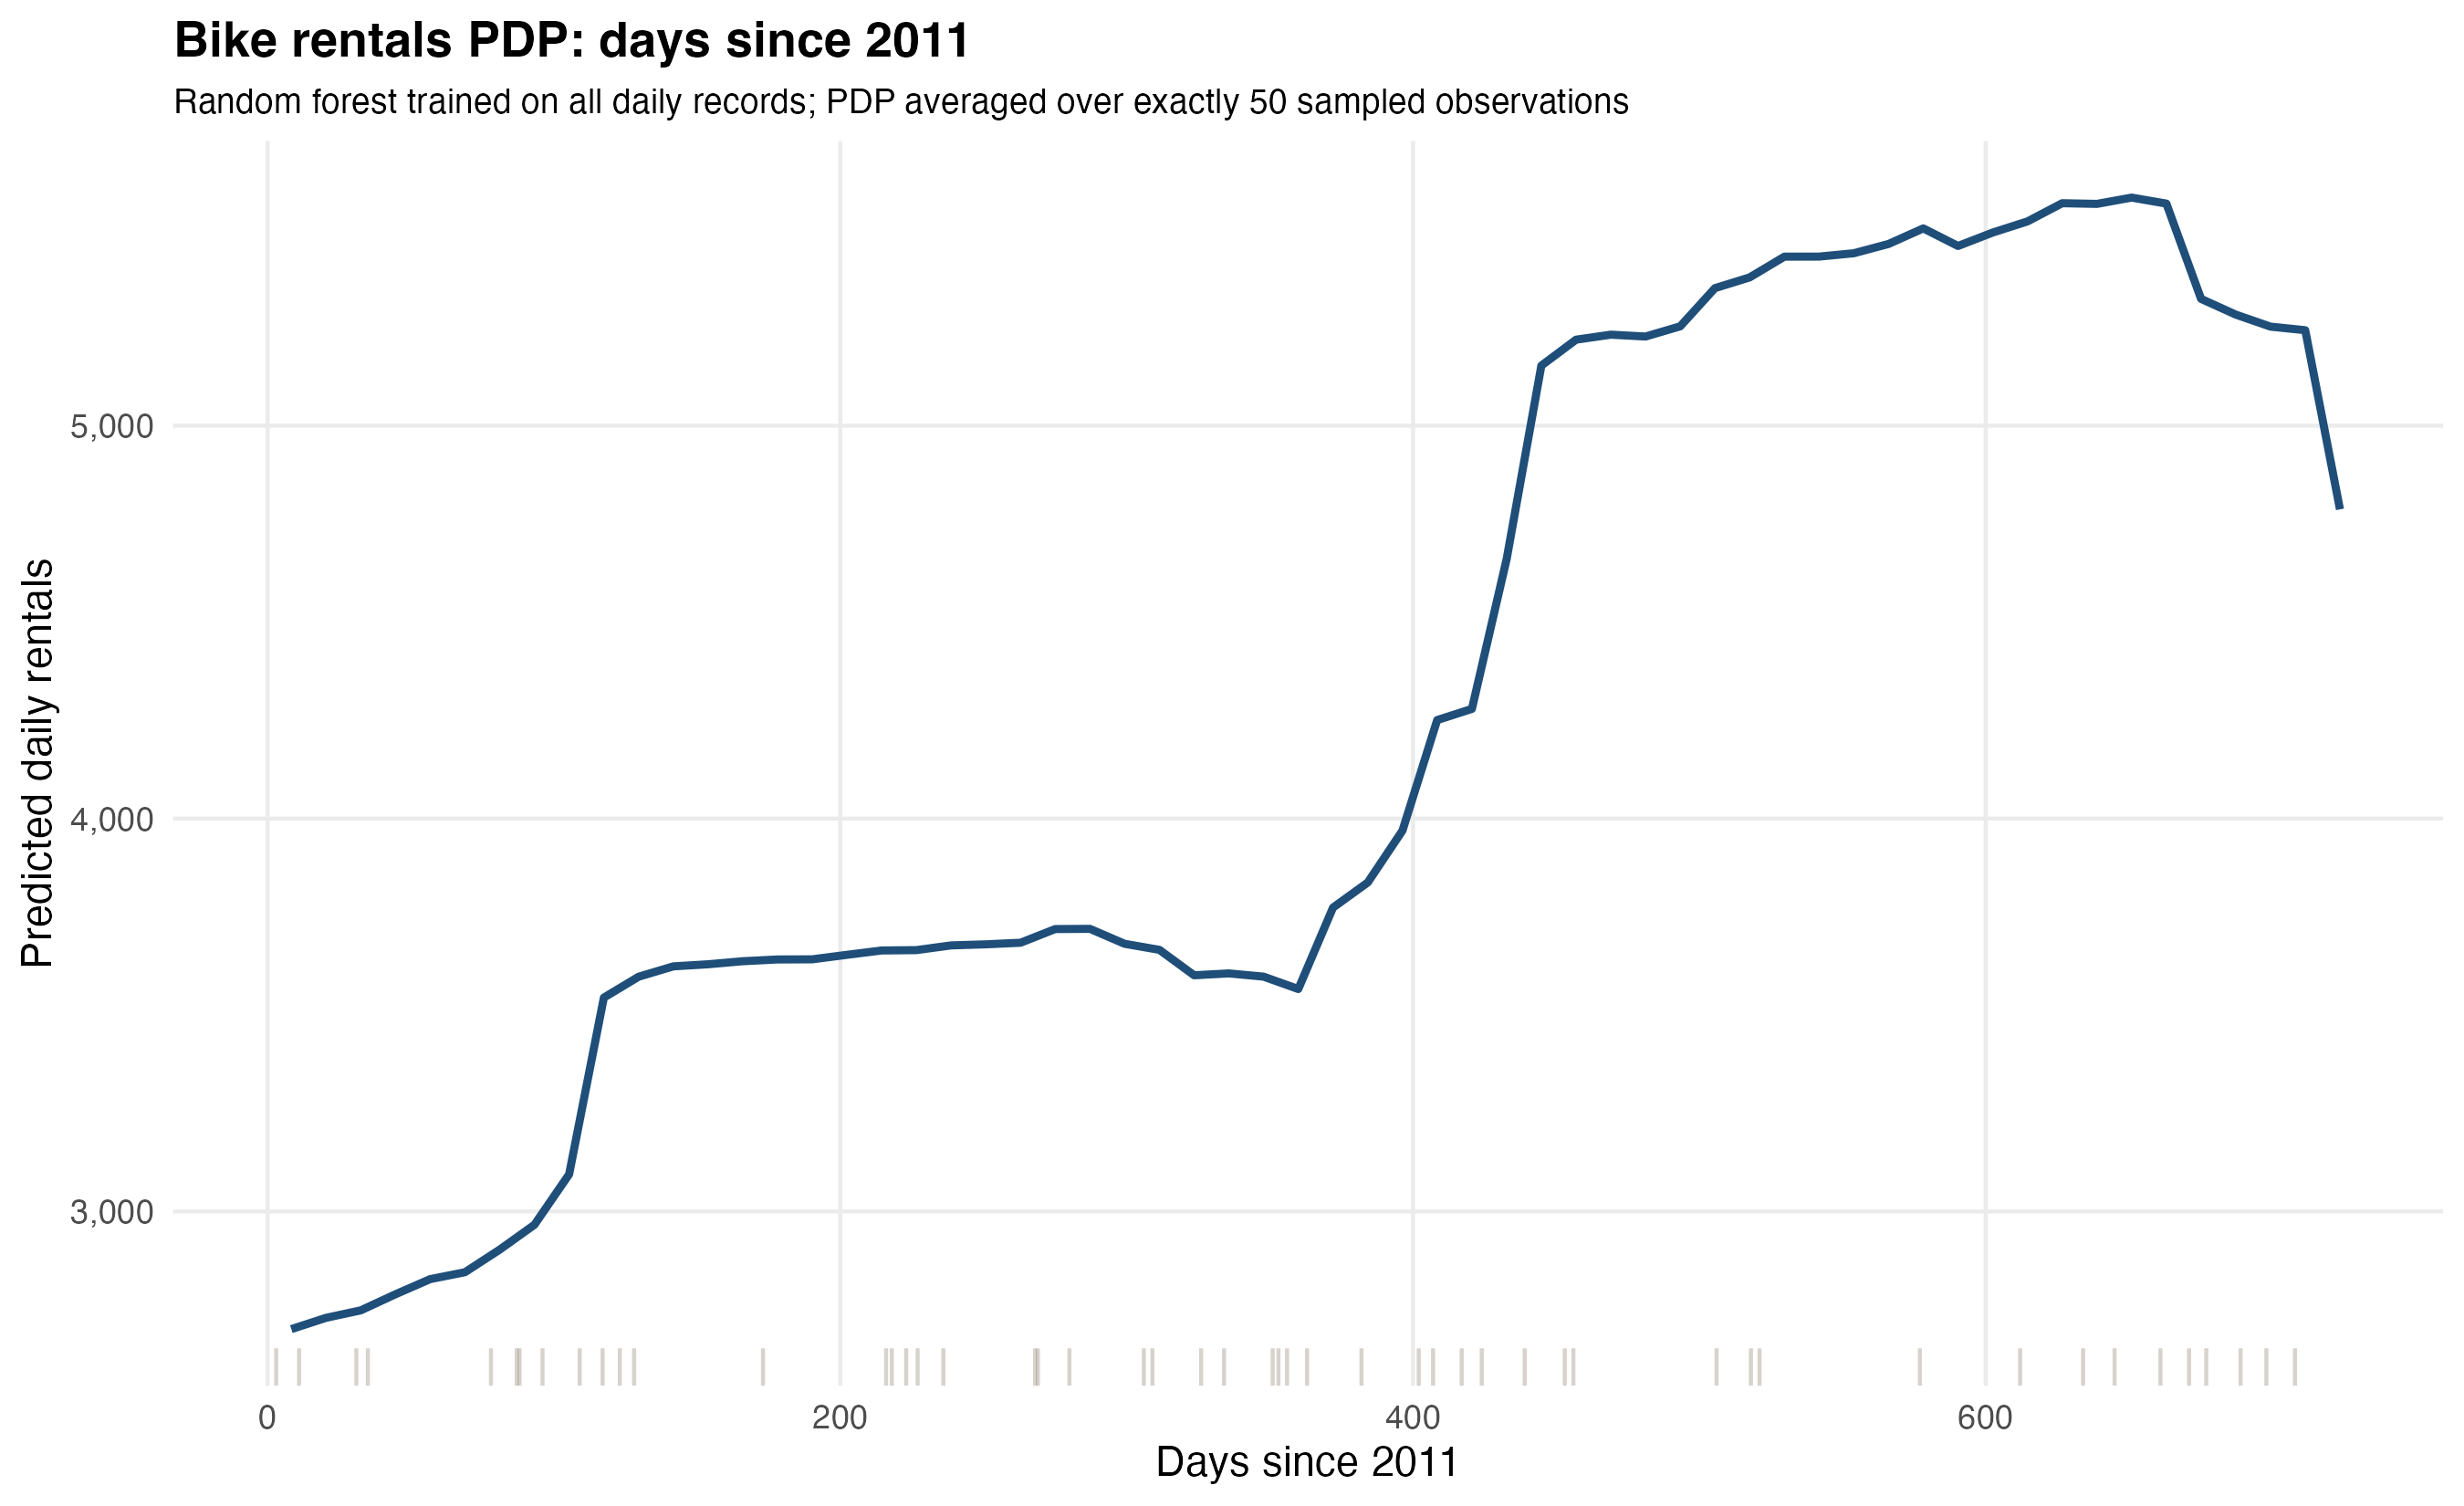
\includegraphics[width=\textwidth]{bike_pdp_days_since_2011.png}
\end{minipage}
\begin{minipage}{0.48\textwidth}
\centering
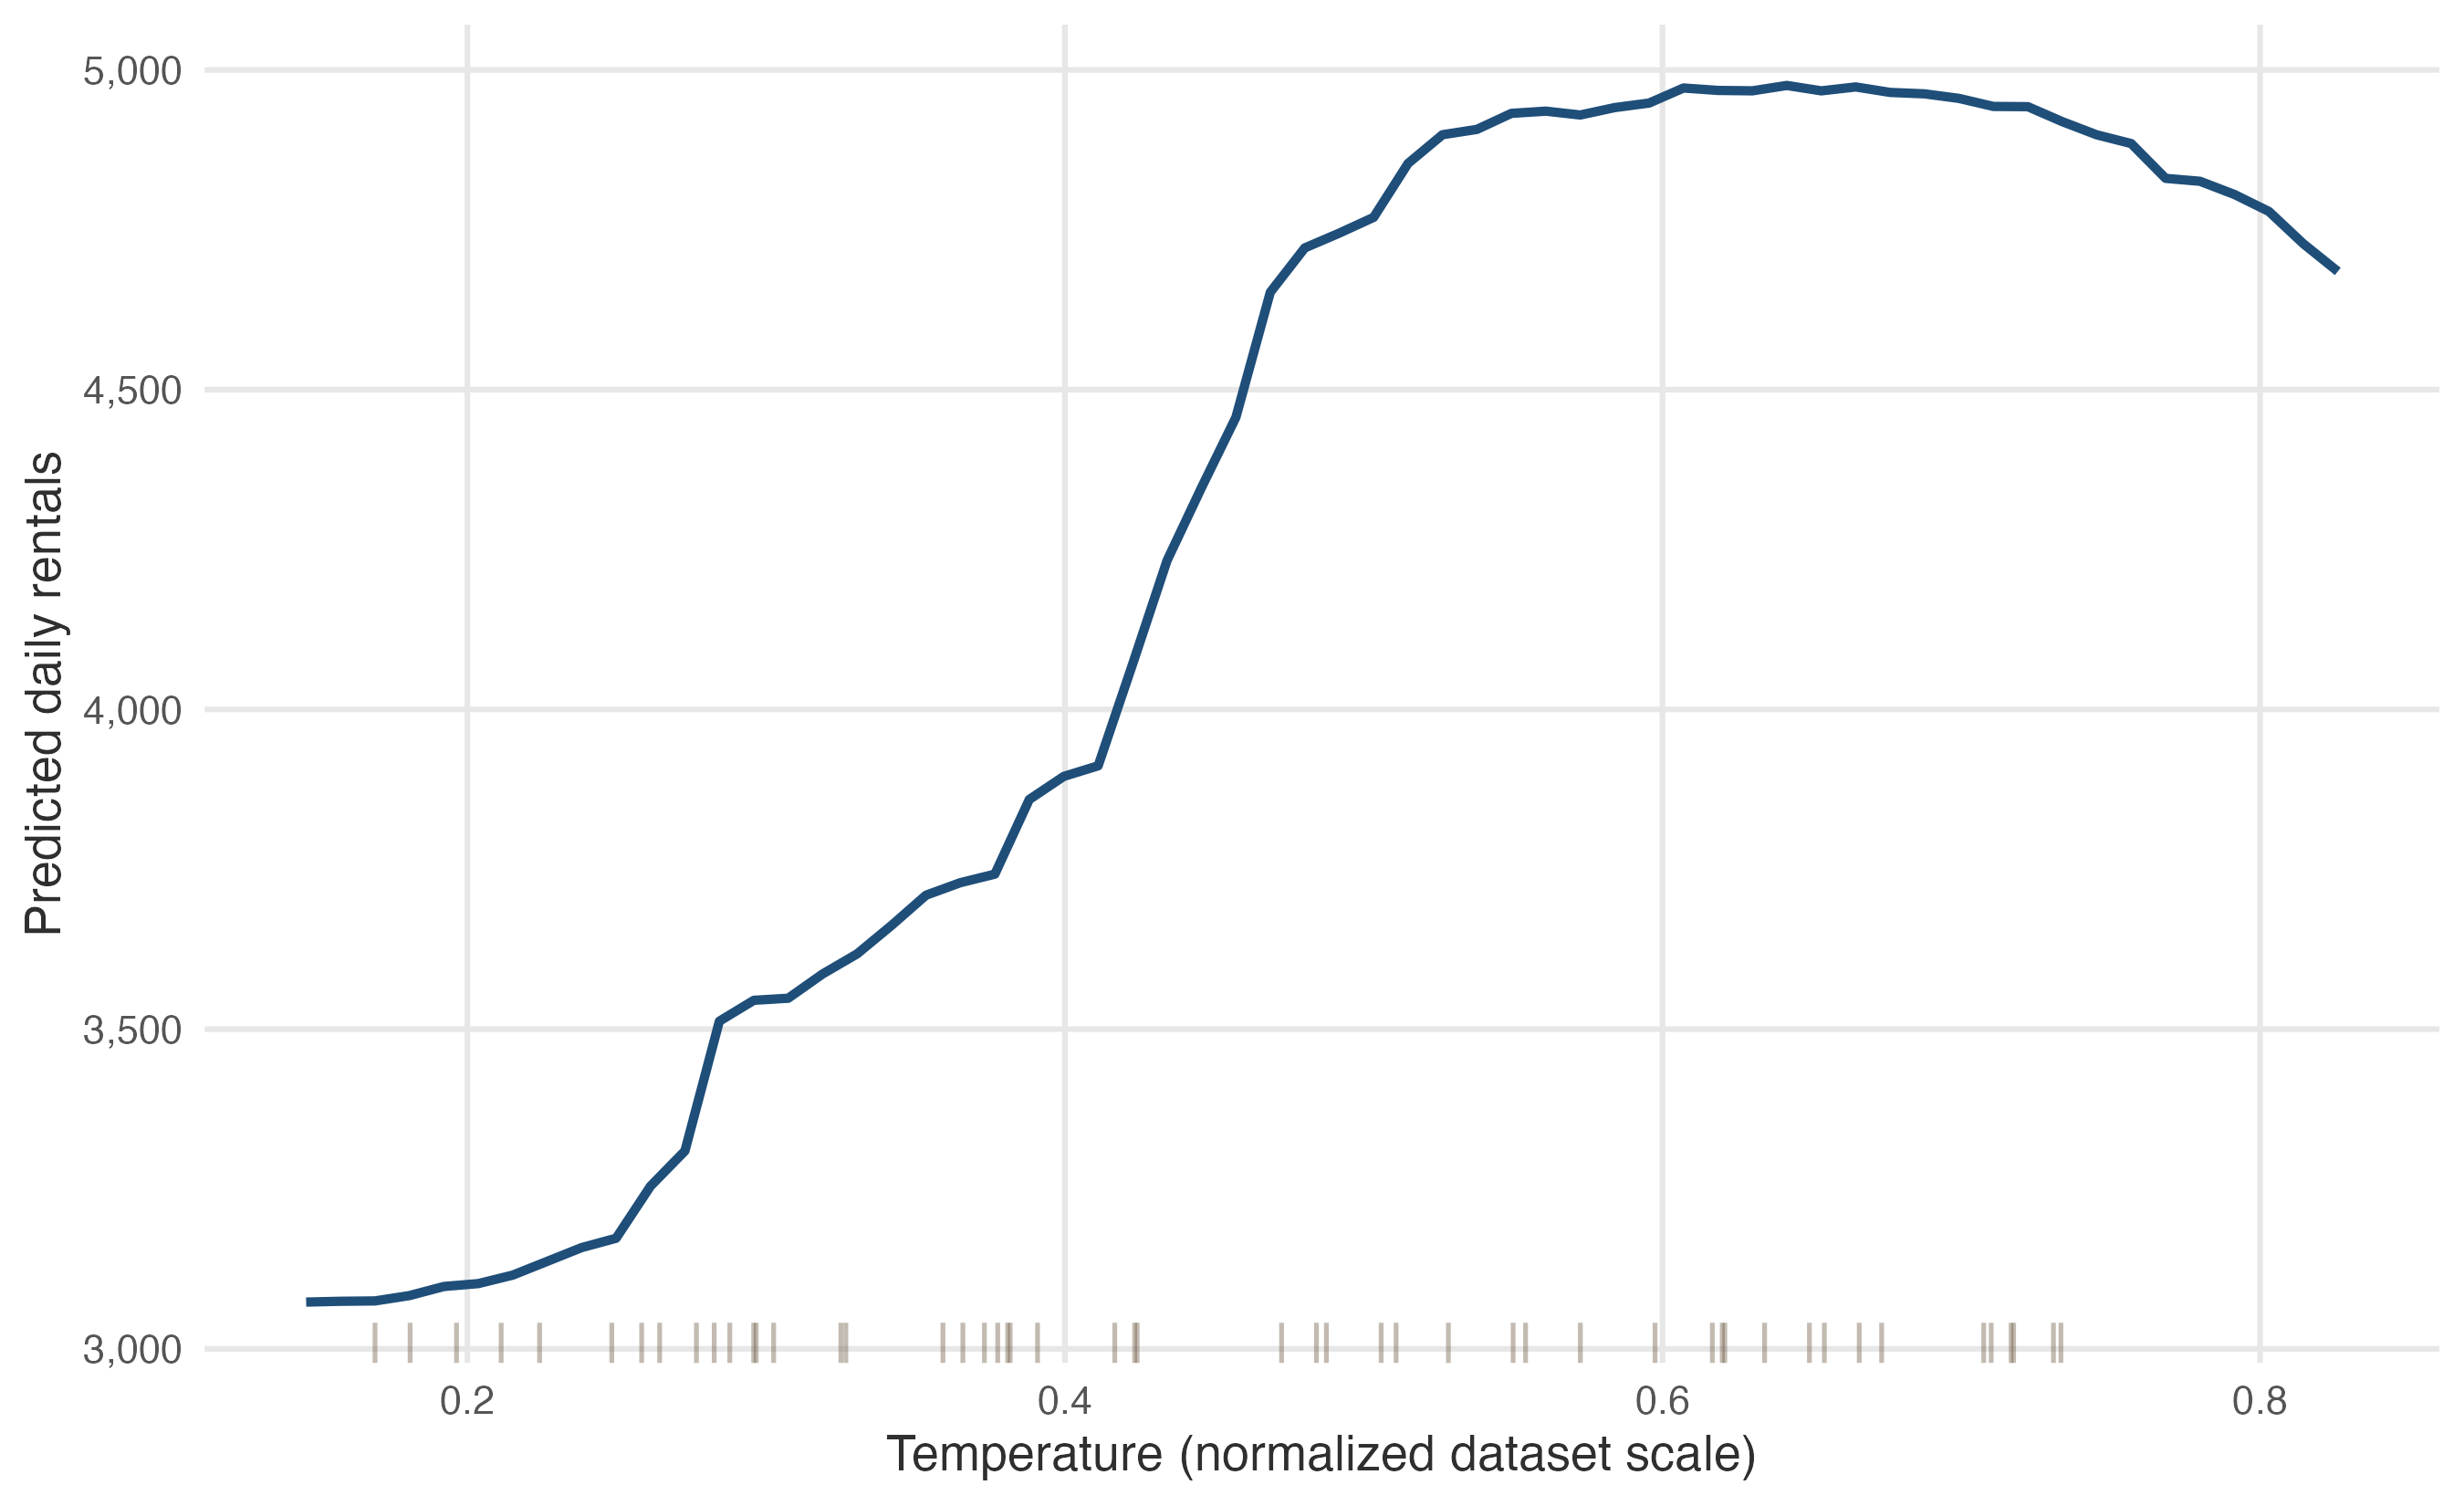
\includegraphics[width=\textwidth]{bike_pdp_temperature.png}
\end{minipage}

\begin{minipage}{0.48\textwidth}
\centering
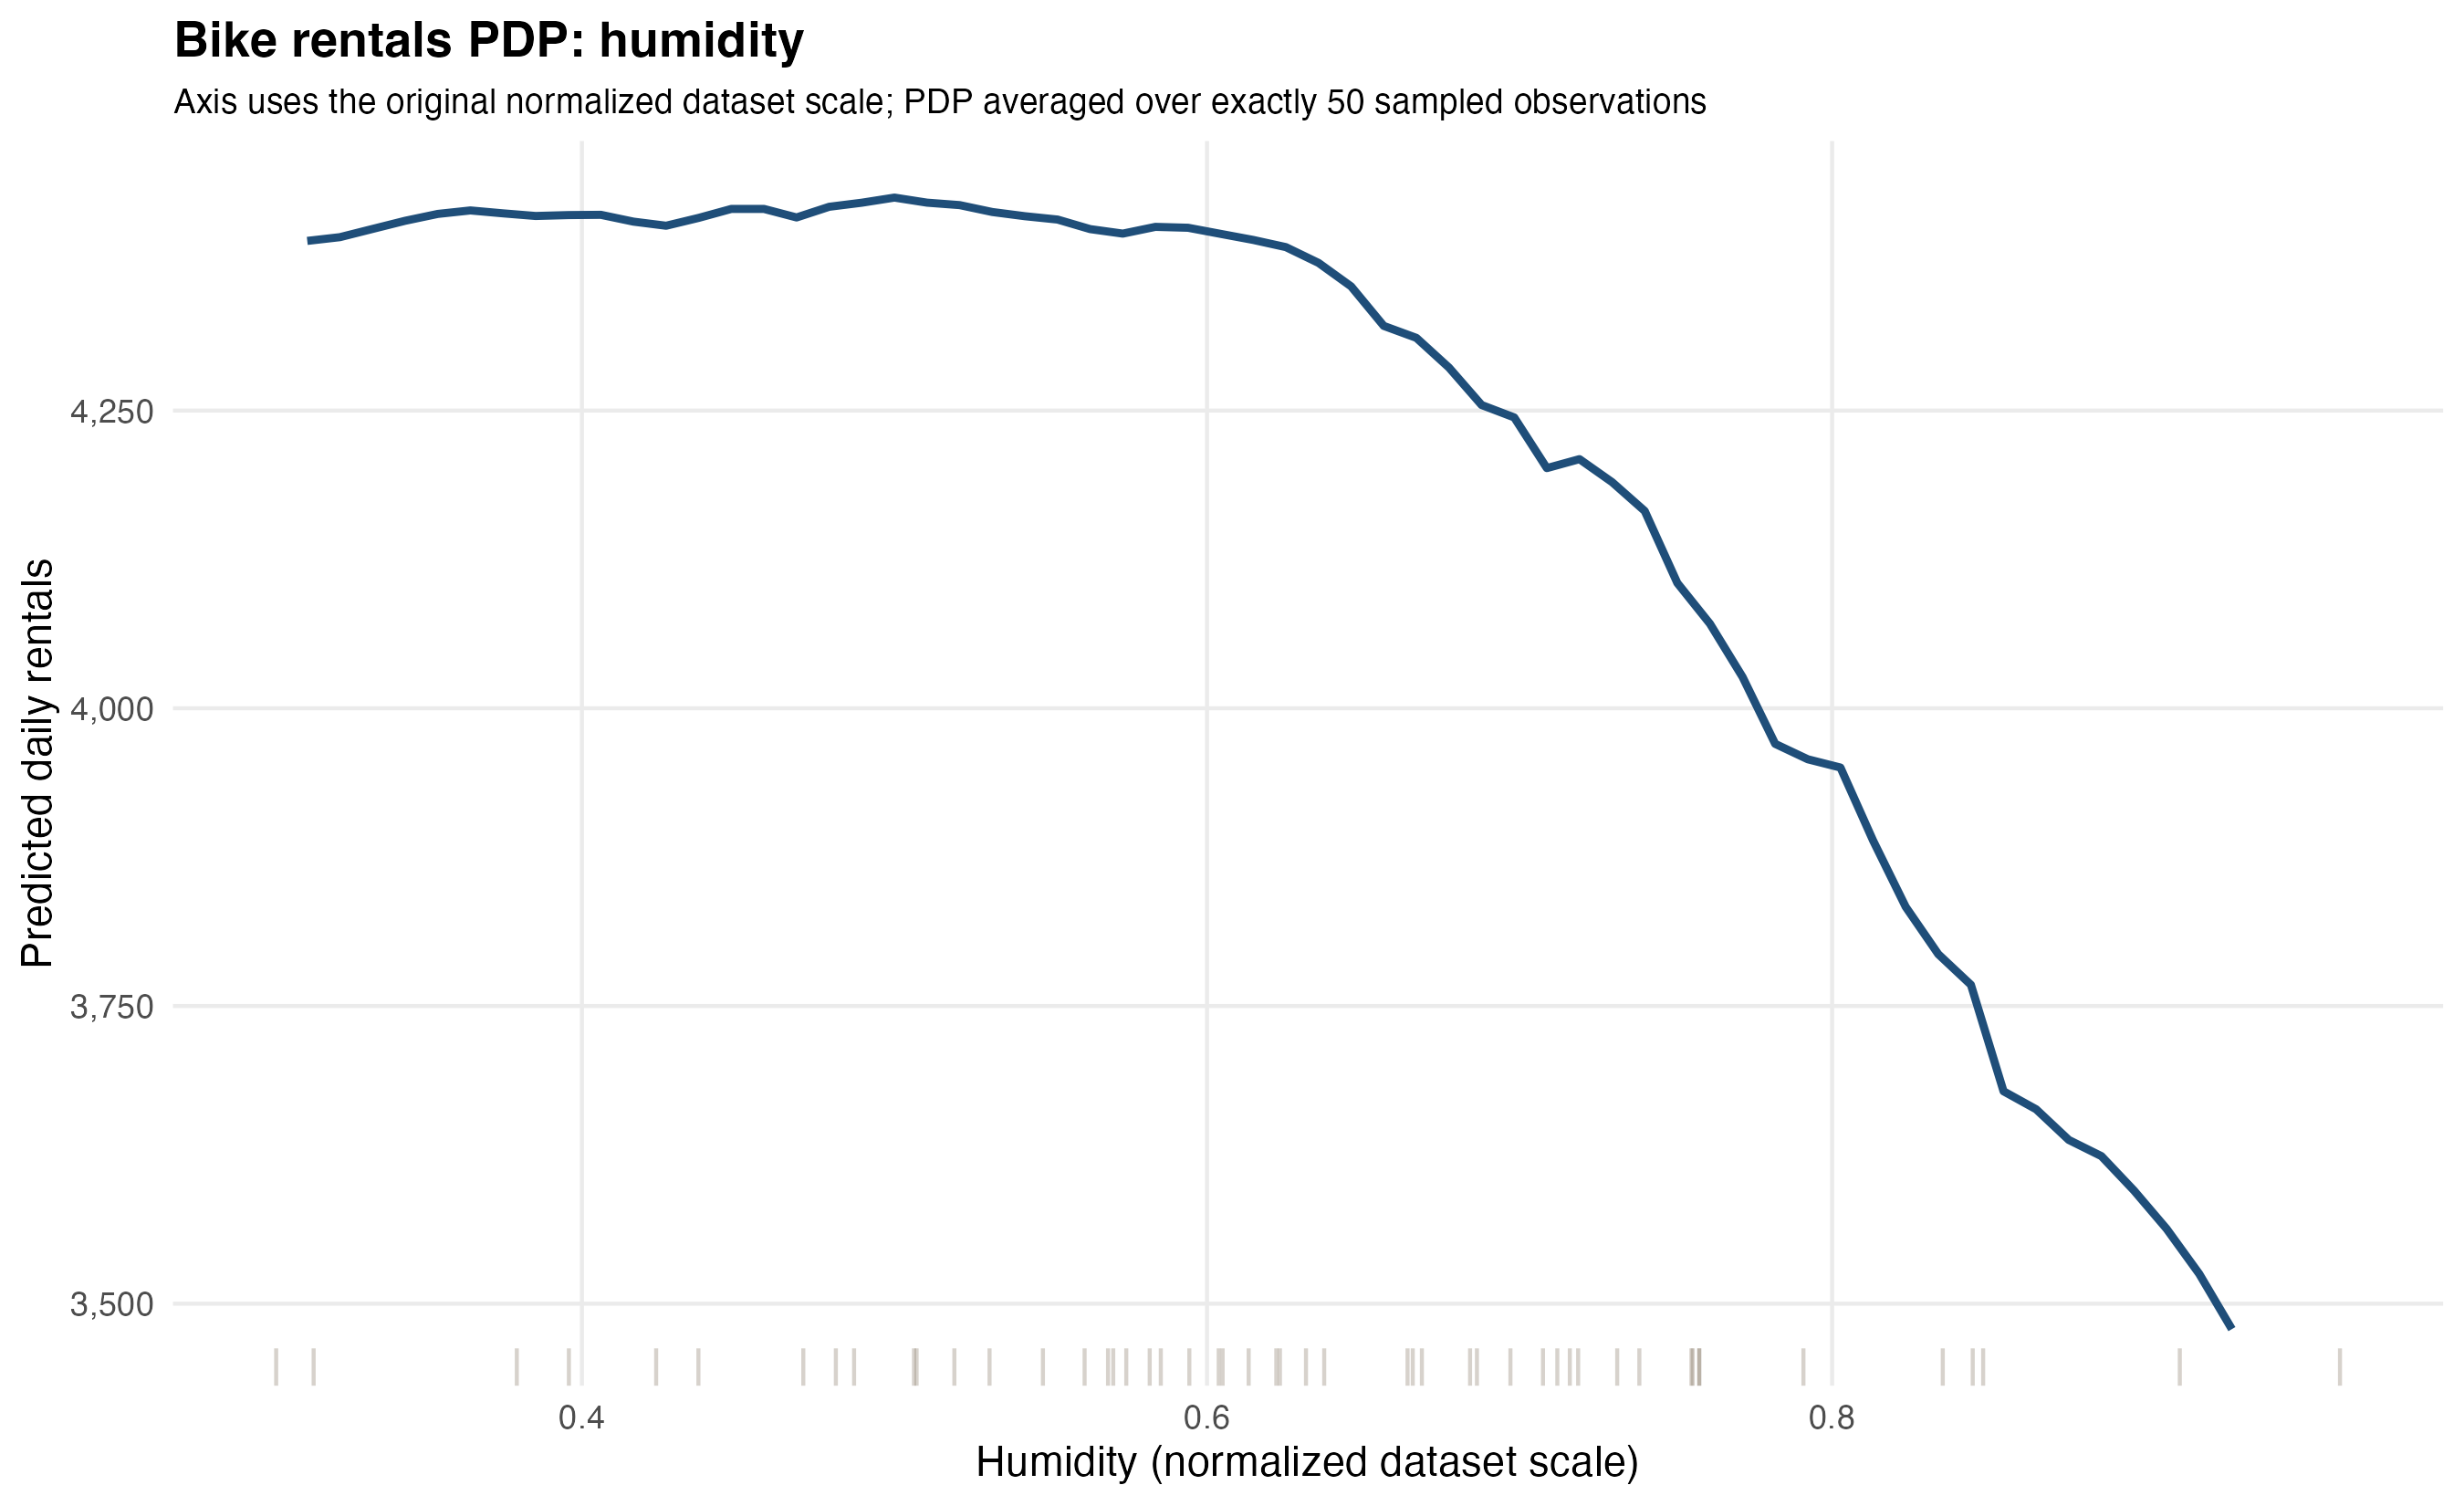
\includegraphics[width=\textwidth]{bike_pdp_humidity.png}
\end{minipage}
\begin{minipage}{0.48\textwidth}
\centering
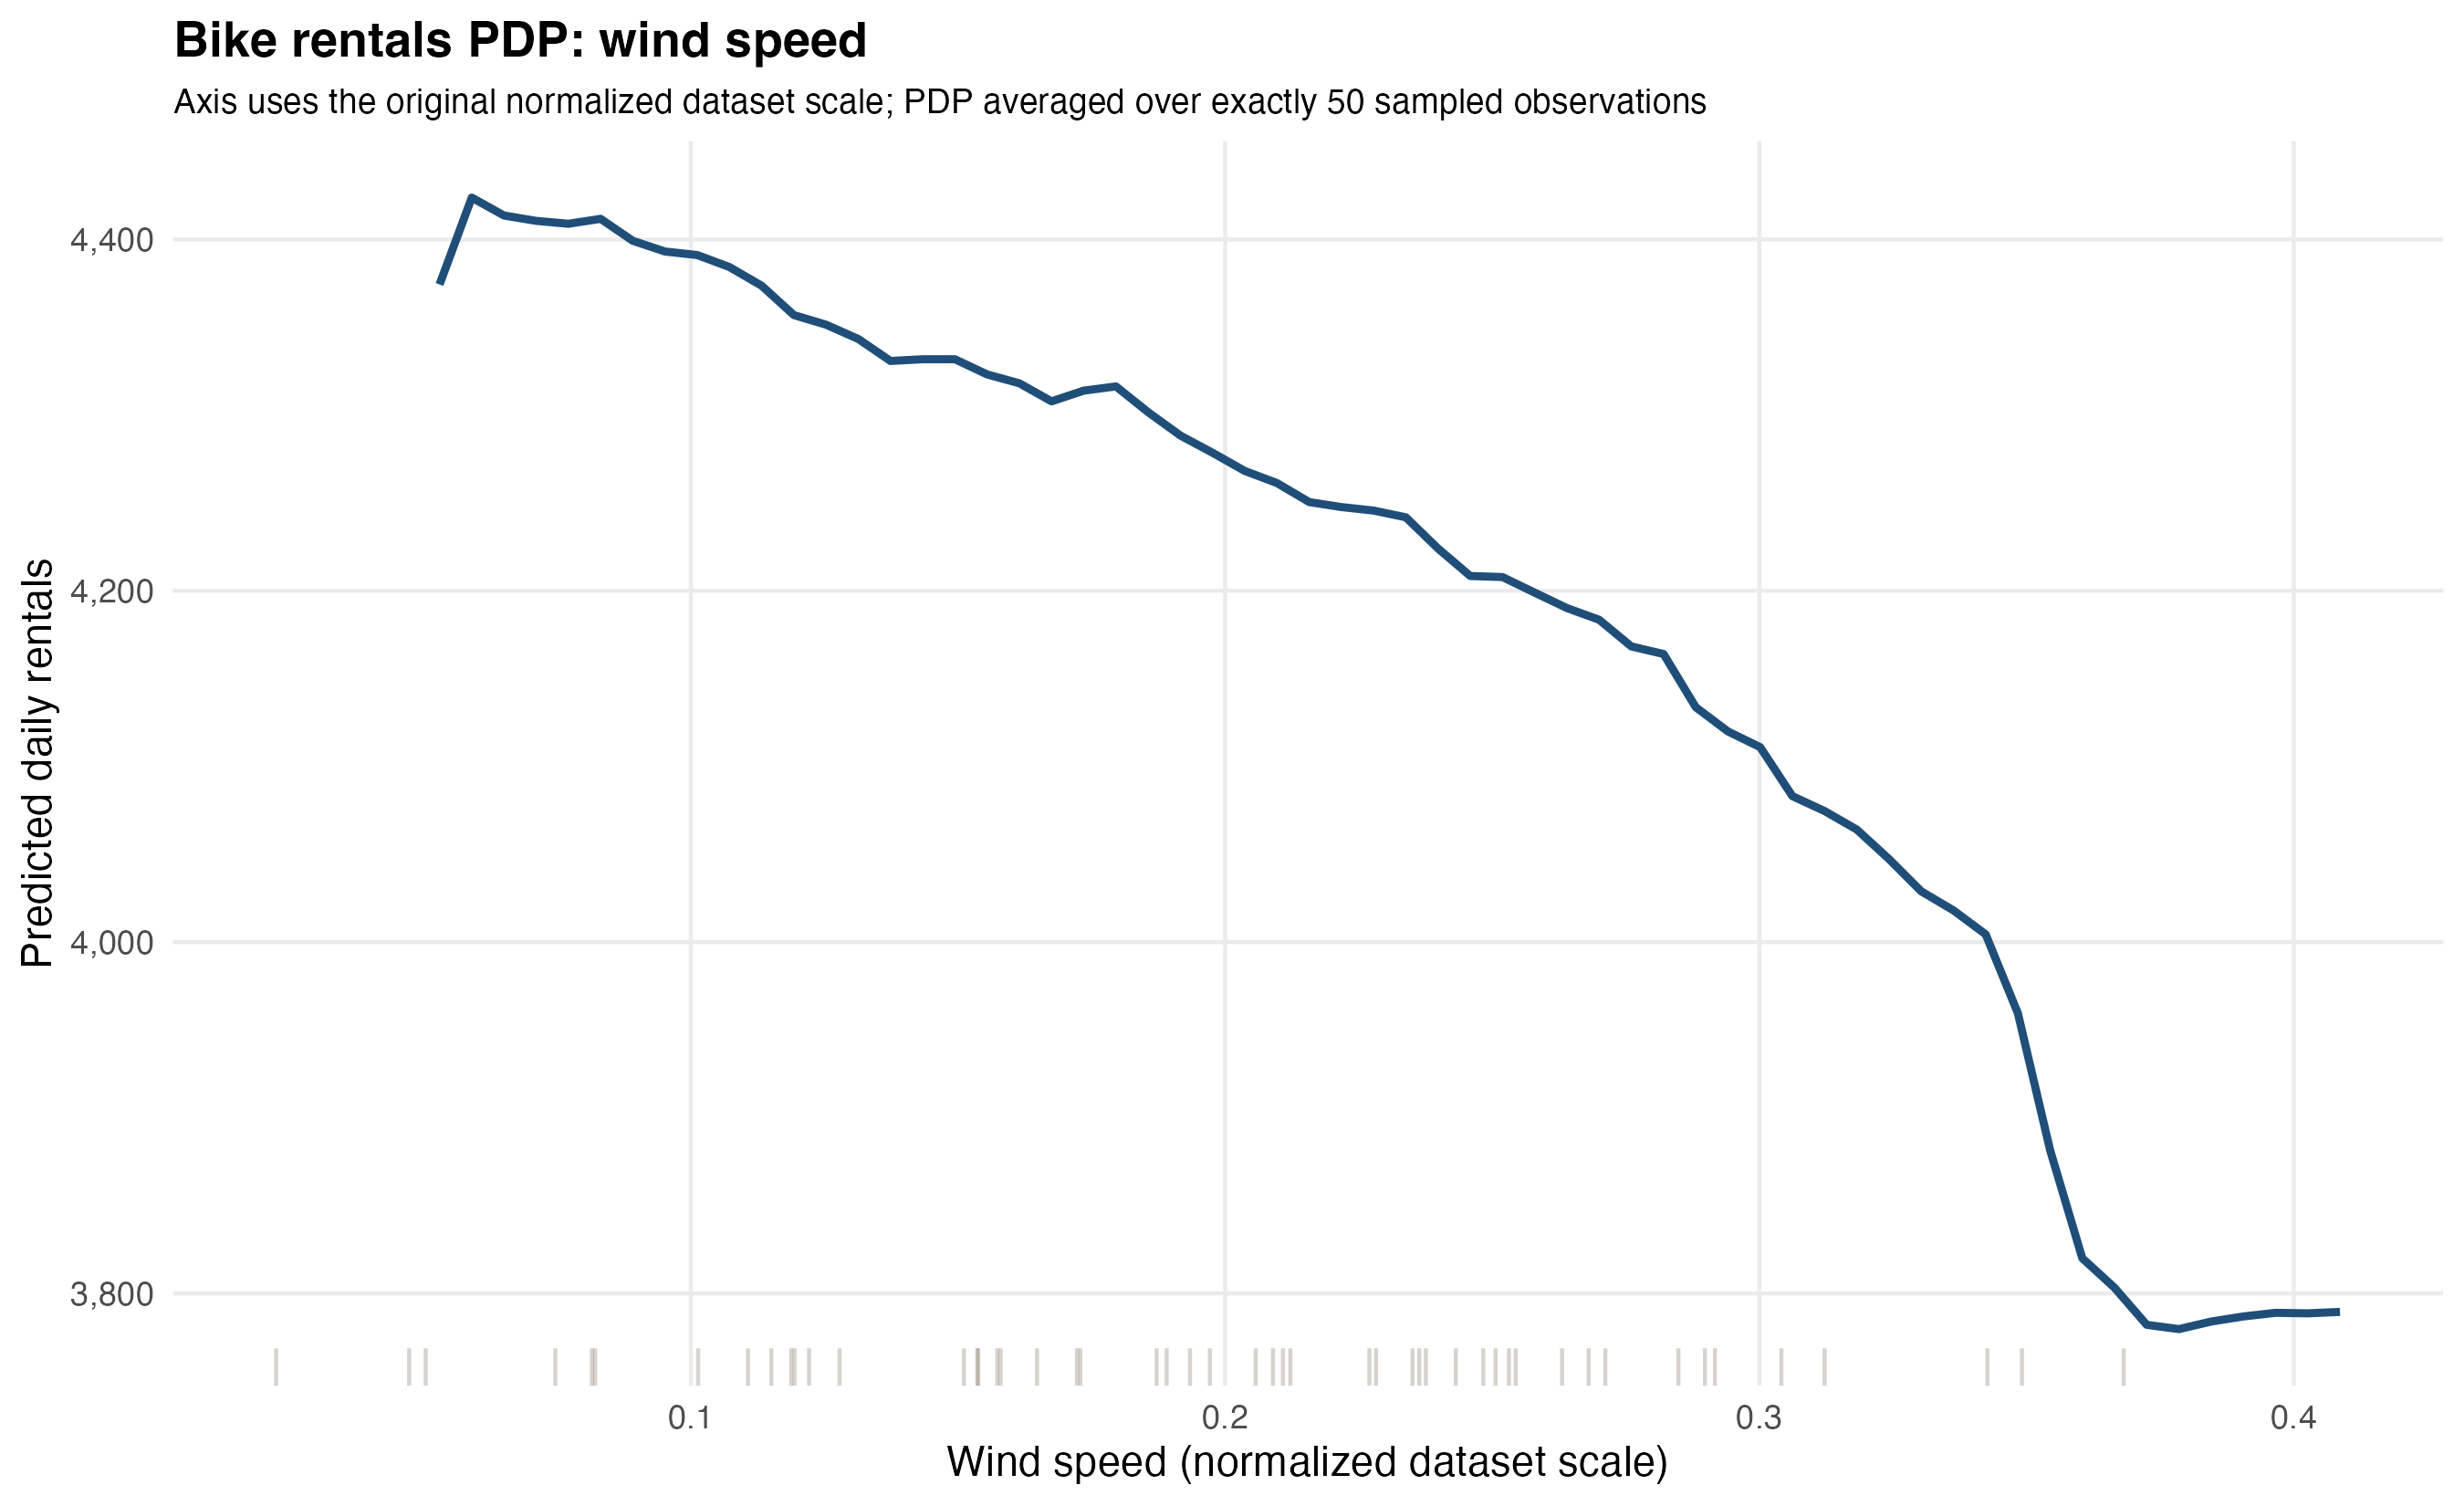
\includegraphics[width=\textwidth]{bike_pdp_windspeed.png}
\end{minipage}
\caption{One-dimensional PDPs for daily bike rental demand. Weather variables are shown on normalized dataset scales.}
\end{figure}

\textbf{Days since 2011.} The model predicts higher demand later in the observed period. The PDP minimum is about 2,701 rentals near day 8, while the maximum is about 5,581 rentals near day 651. For a bike rental operator, this indicates that the model has learned an adoption or maturity pattern across the time series. Fleet sizing, staffing, and maintenance capacity should account for this higher baseline demand in the later part of the historical period.

\textbf{Temperature, normalized.} Temperature has a strong positive effect until the medium-high part of the normalized scale. Predicted demand rises from about 3,073 rentals at normalized temperature 0.15 to about 4,976 rentals around 0.64. After that point the curve flattens and slightly declines. Operationally, warm but not extreme days should be treated as high-demand days.

\textbf{Humidity, normalized.} Humidity has a negative relationship with predicted rentals at the high end of the normalized scale. The PDP reaches about 4,429 rentals near normalized humidity 0.50, but falls to about 3,479 rentals near 0.93. High humidity should therefore reduce demand expectations.

\textbf{Wind speed, normalized.} Wind speed also reduces predicted demand. The model predicts about 4,424 rentals at low normalized wind speed, near 0.06, and about 3,780 rentals near 0.38. This effect is smaller than the temperature and time effects, but it is still useful for daily demand adjustment.

\subsection{Two-Dimensional Temperature and Humidity PDP}

\begin{figure}[H]
\centering
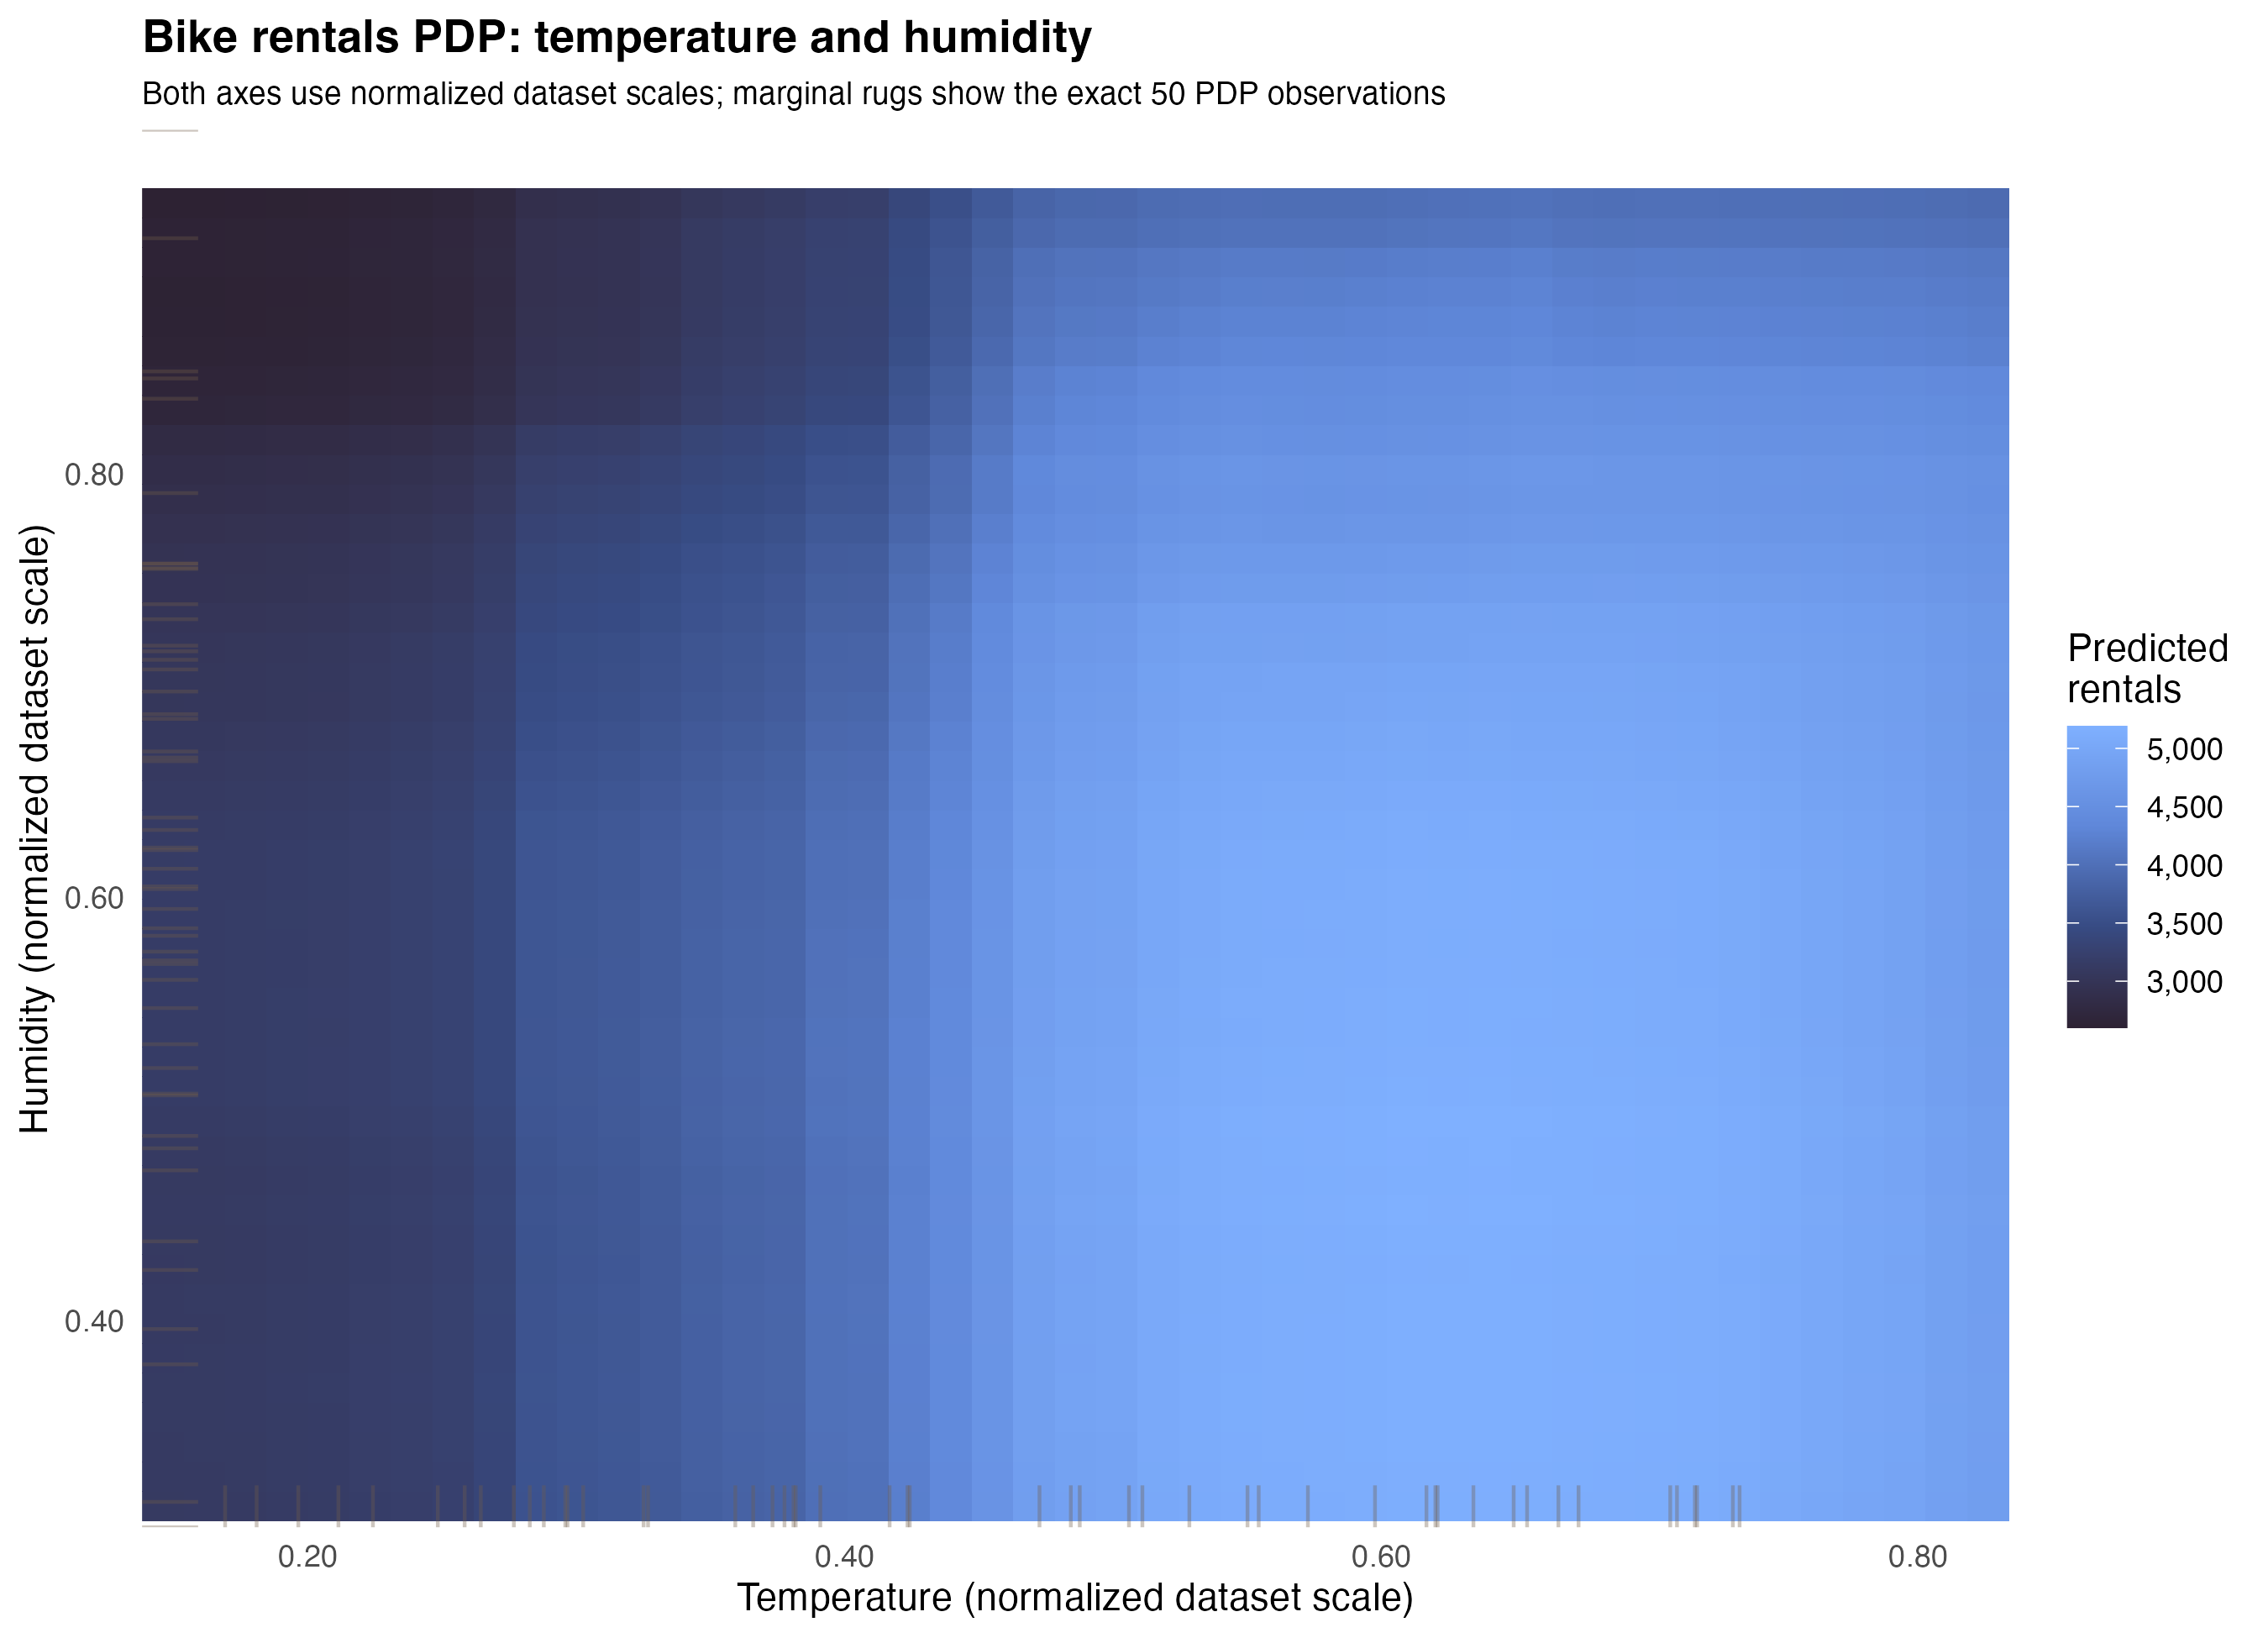
\includegraphics[width=0.95\textwidth]{bike_pdp_2d_temperature_humidity_heatmap.png}
\caption{Two-dimensional PDP for normalized temperature and normalized humidity. Marginal rugs show the exact 50 observations used for PDP calculation.}
\end{figure}

The two-dimensional PDP answers the assignment question about the joint effect of humidity and temperature. The highest predicted demand appears around normalized temperature 0.64 and normalized humidity 0.49, with about 5,190 predicted rentals. The lowest predicted region appears around normalized temperature 0.15 and normalized humidity 0.93, with about 2,601 predicted rentals.

For business planning, temperature should not be interpreted in isolation. Warm conditions are favorable mainly when humidity is moderate. Low temperature combined with high humidity is the weakest demand scenario in the model. The marginal rugs are important because they show where the 50 explanatory observations are located; interpretations are more reliable in regions with observed support.

\section{House Price Prediction}

\begin{figure}[H]
\centering
\begin{minipage}{0.48\textwidth}
\centering
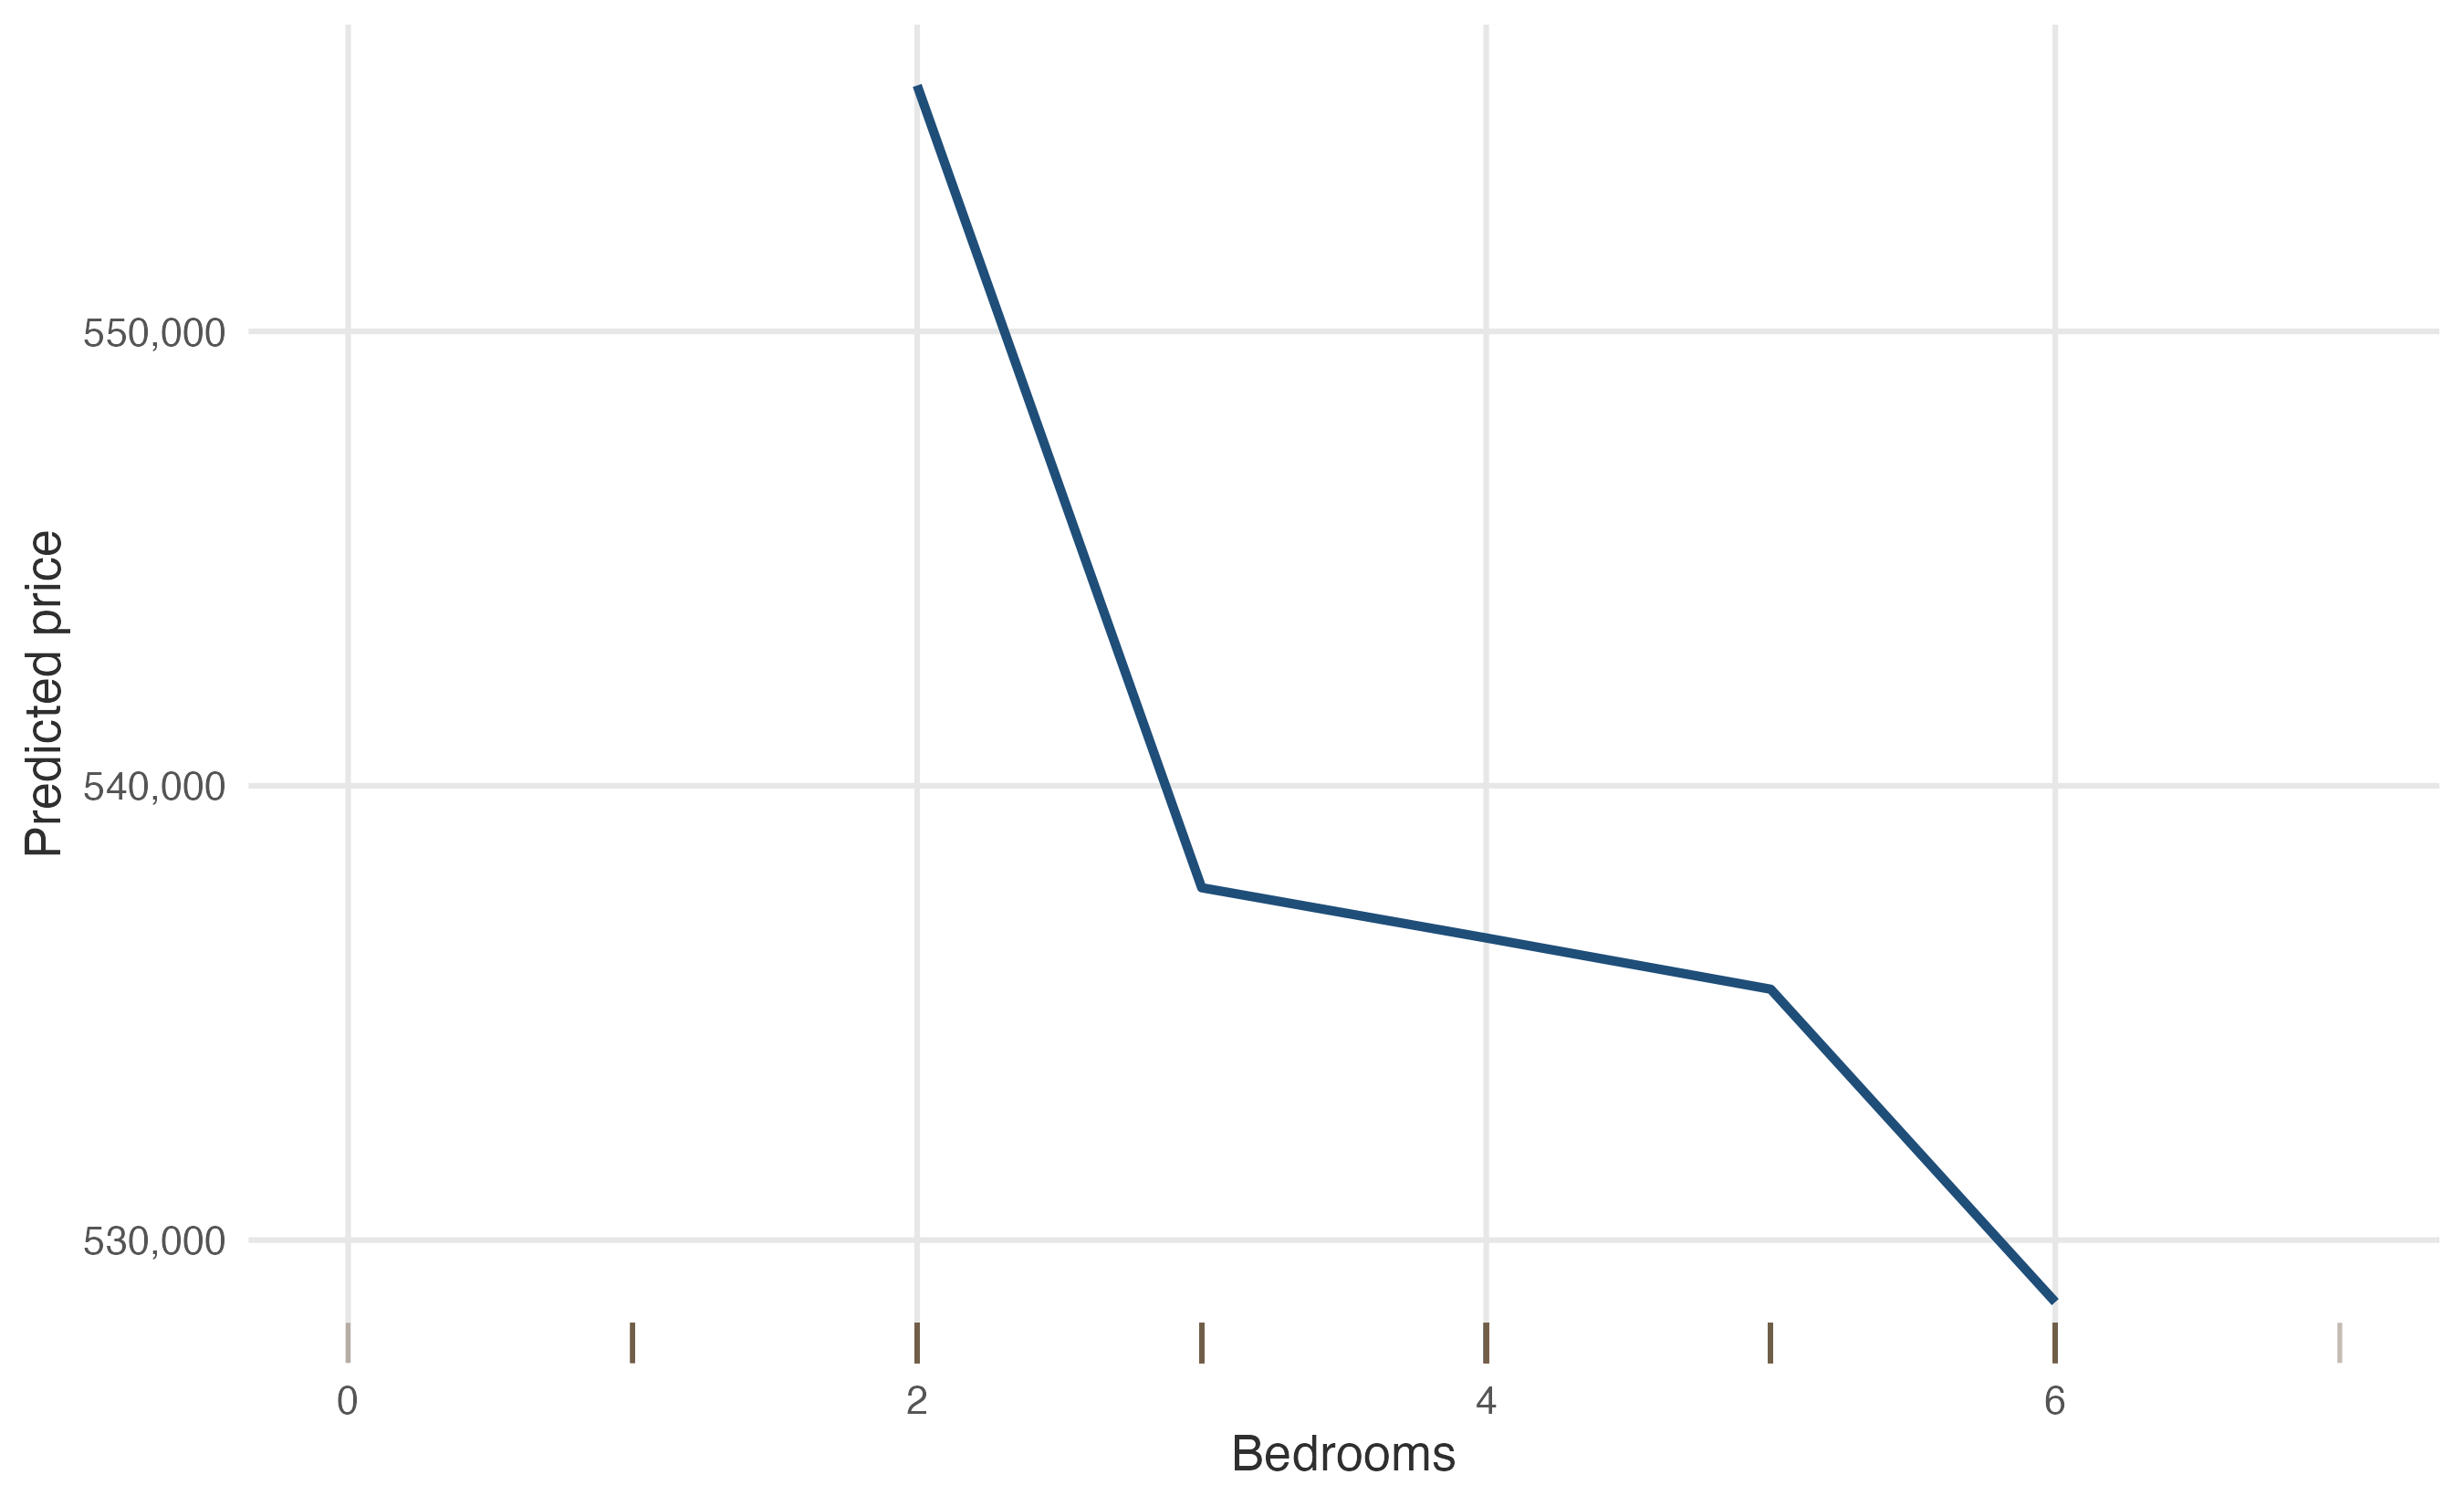
\includegraphics[width=\textwidth]{house_pdp_bedrooms.png}
\end{minipage}
\begin{minipage}{0.48\textwidth}
\centering
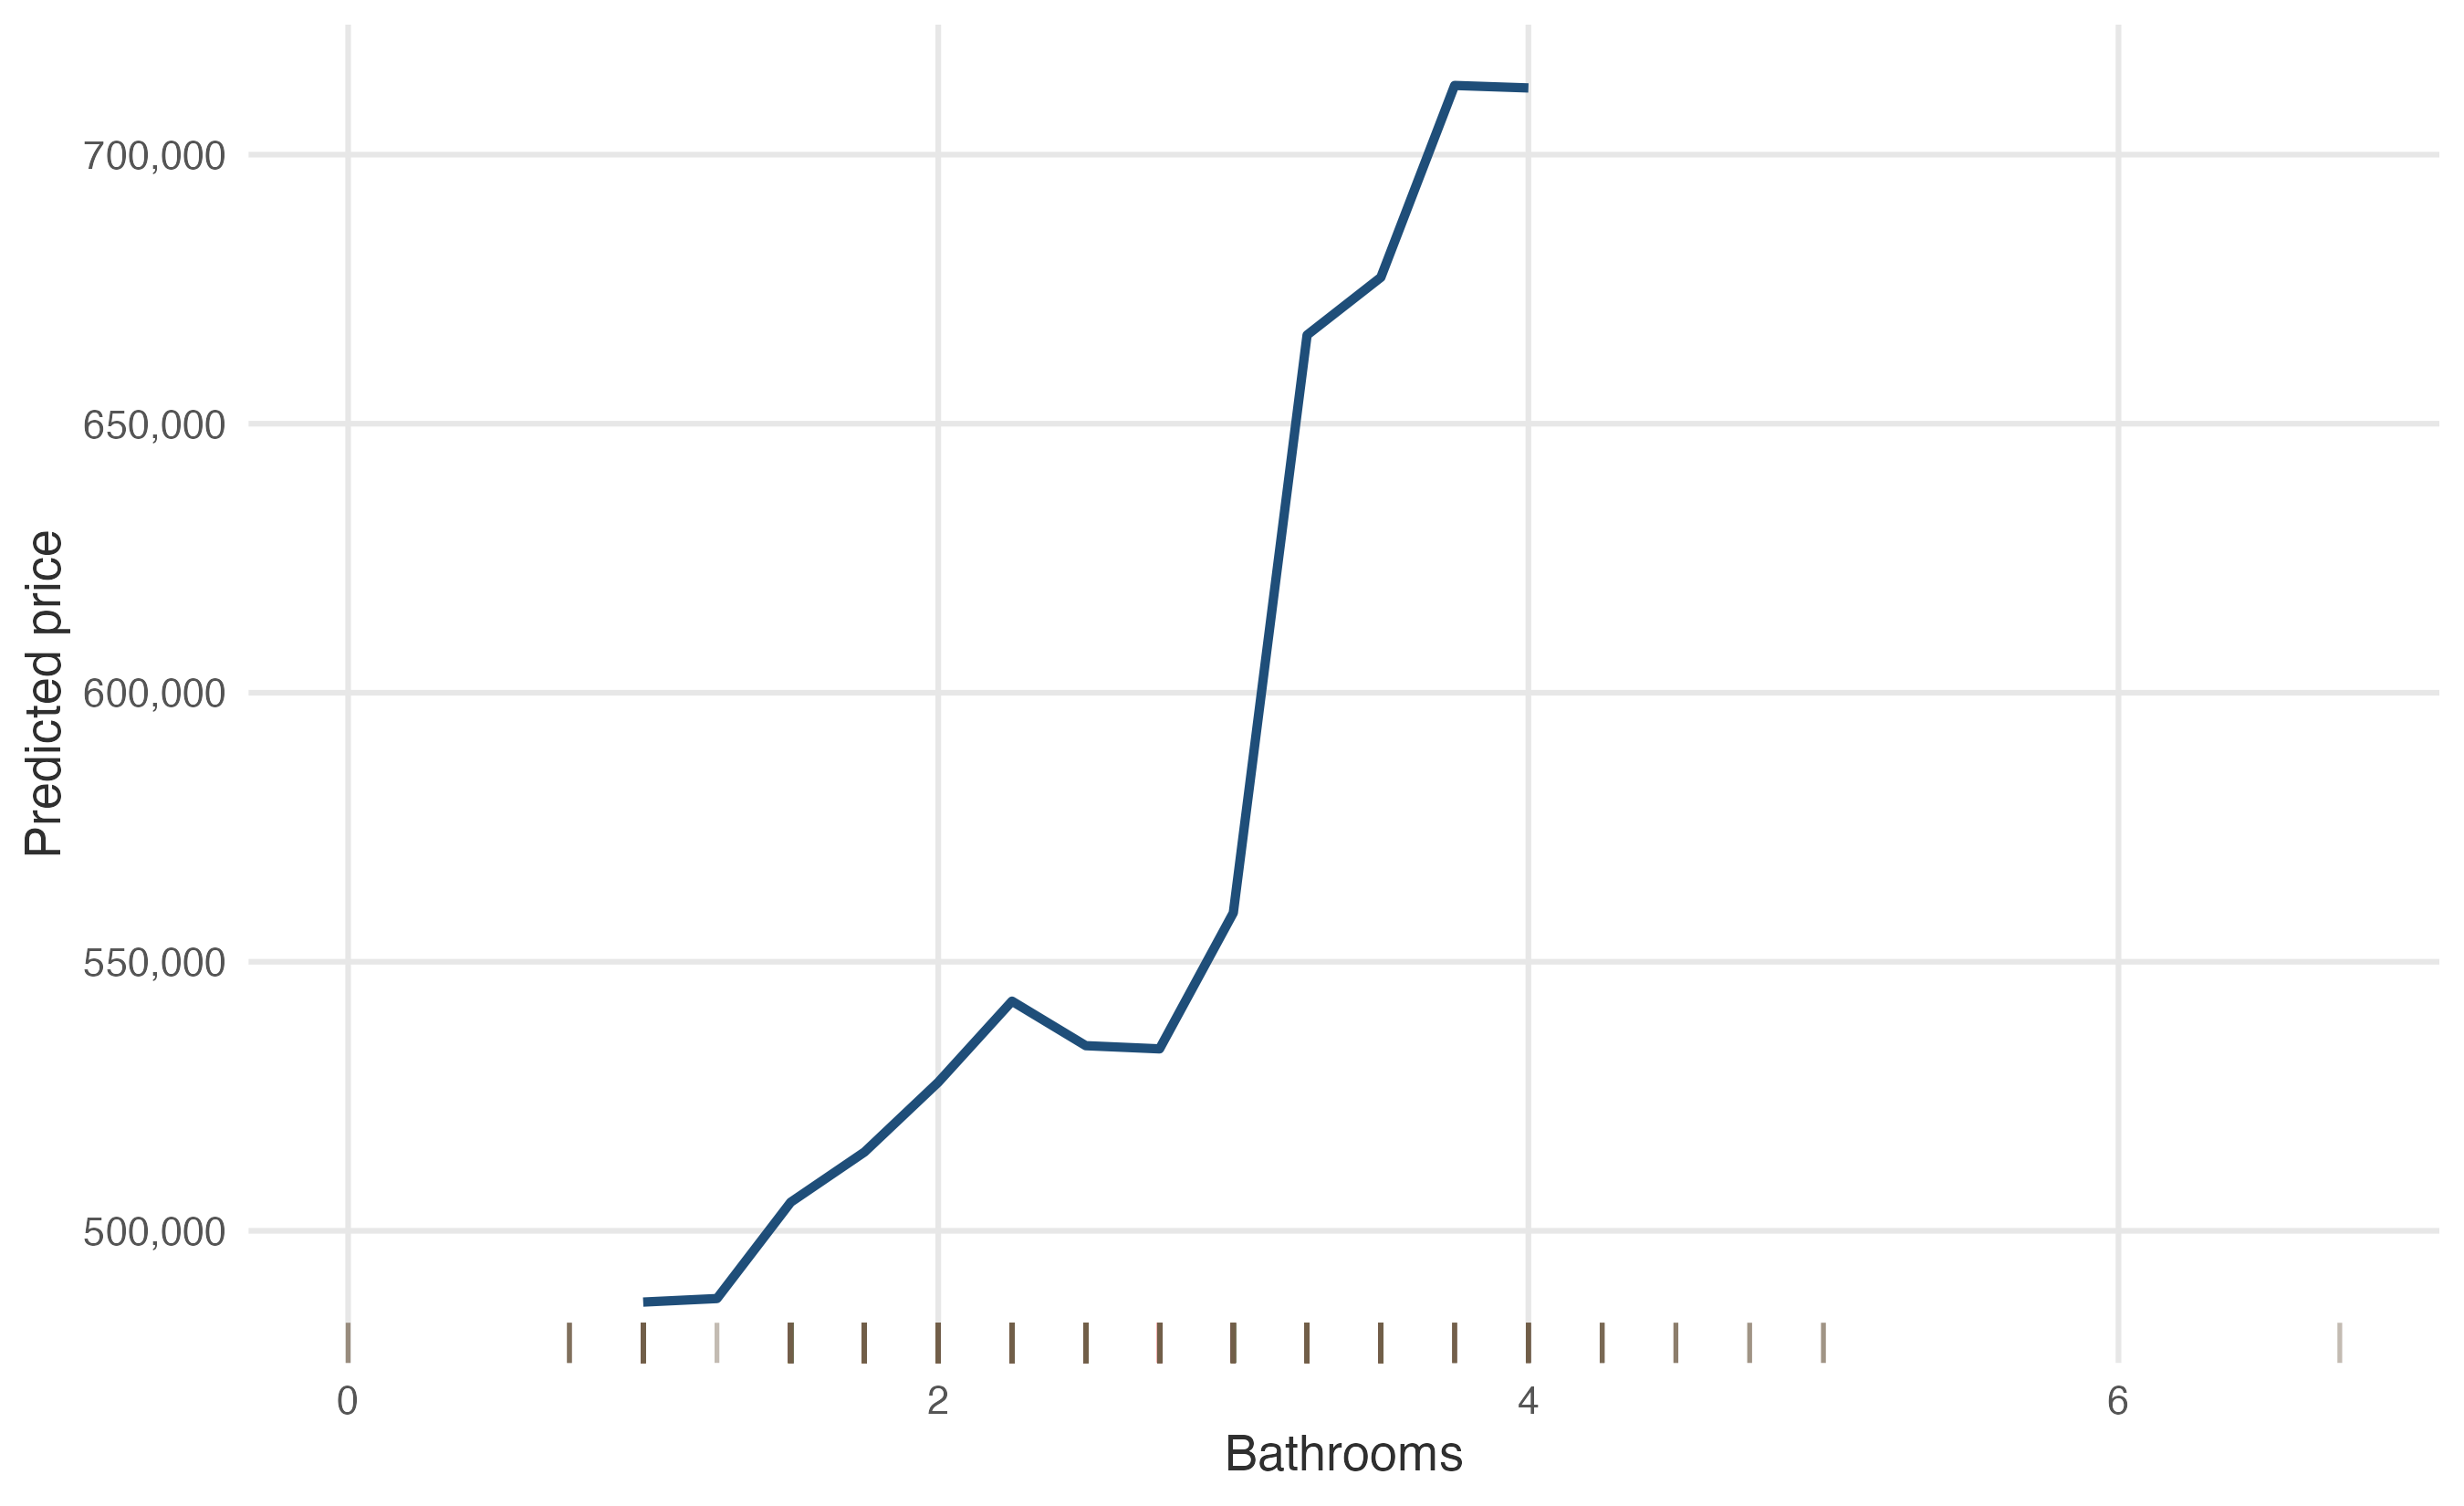
\includegraphics[width=\textwidth]{house_pdp_bathrooms.png}
\end{minipage}

\begin{minipage}{0.48\textwidth}
\centering
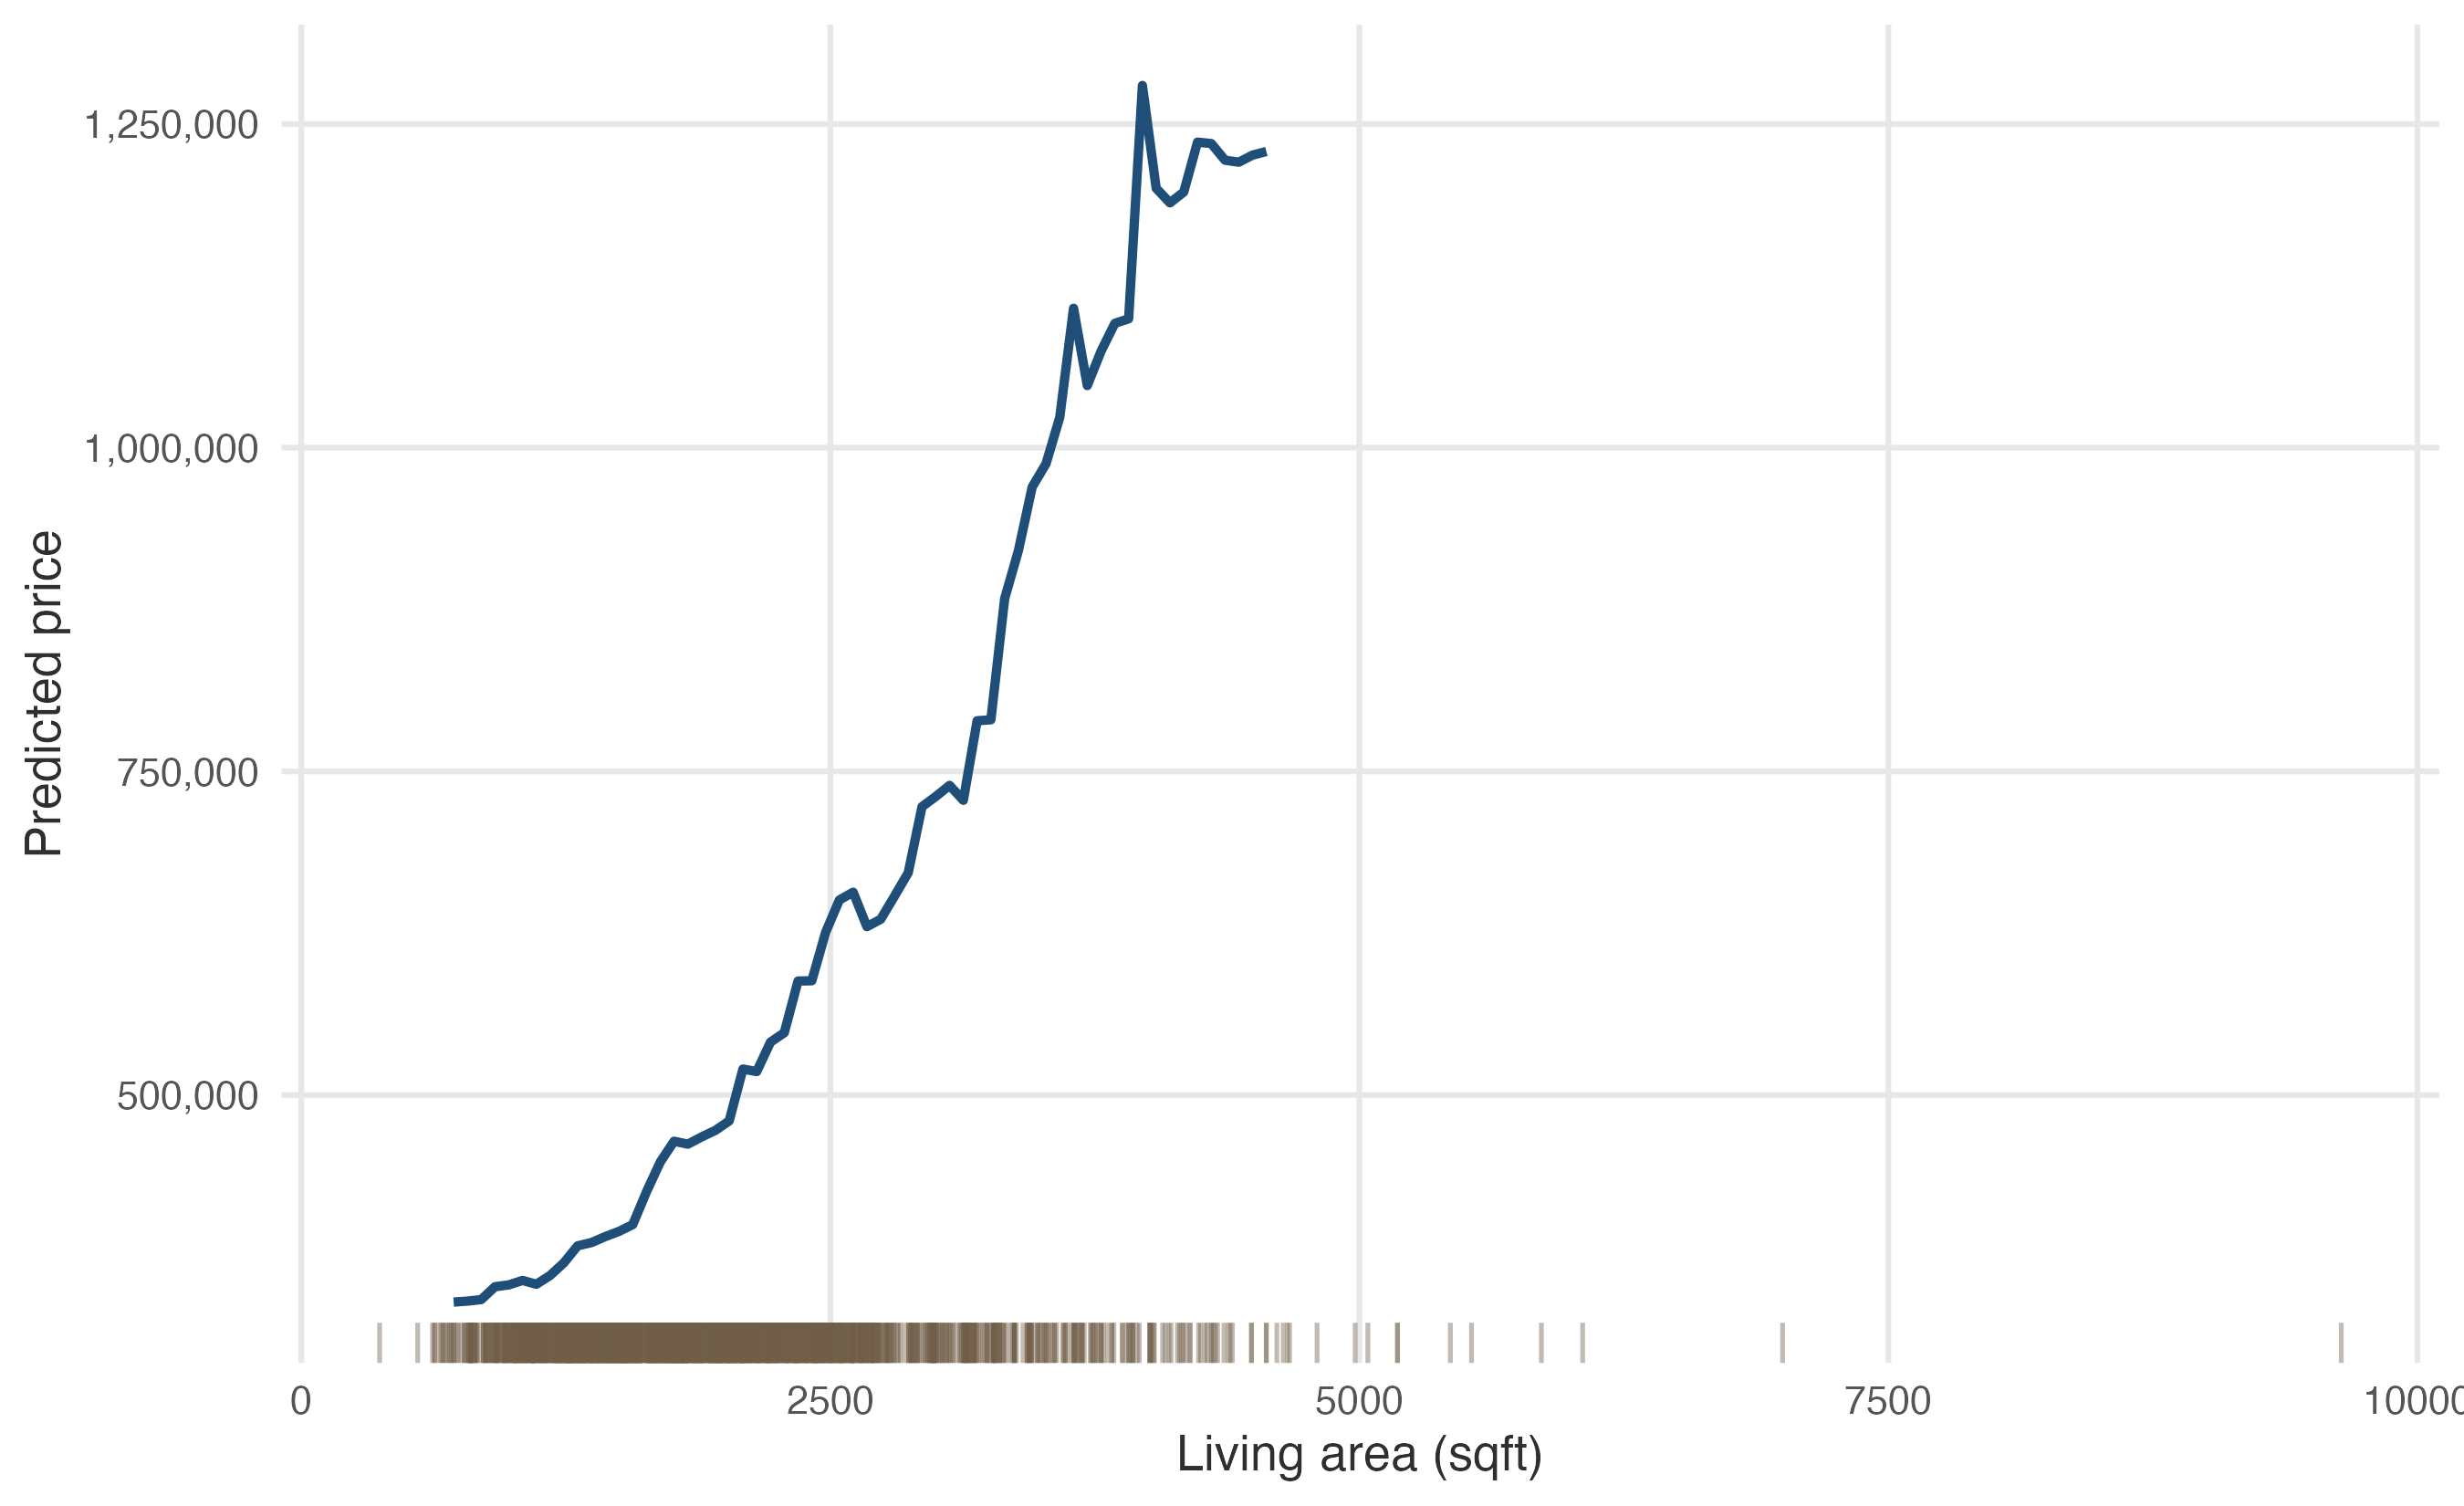
\includegraphics[width=\textwidth]{house_pdp_sqft_living.png}
\end{minipage}
\begin{minipage}{0.48\textwidth}
\centering
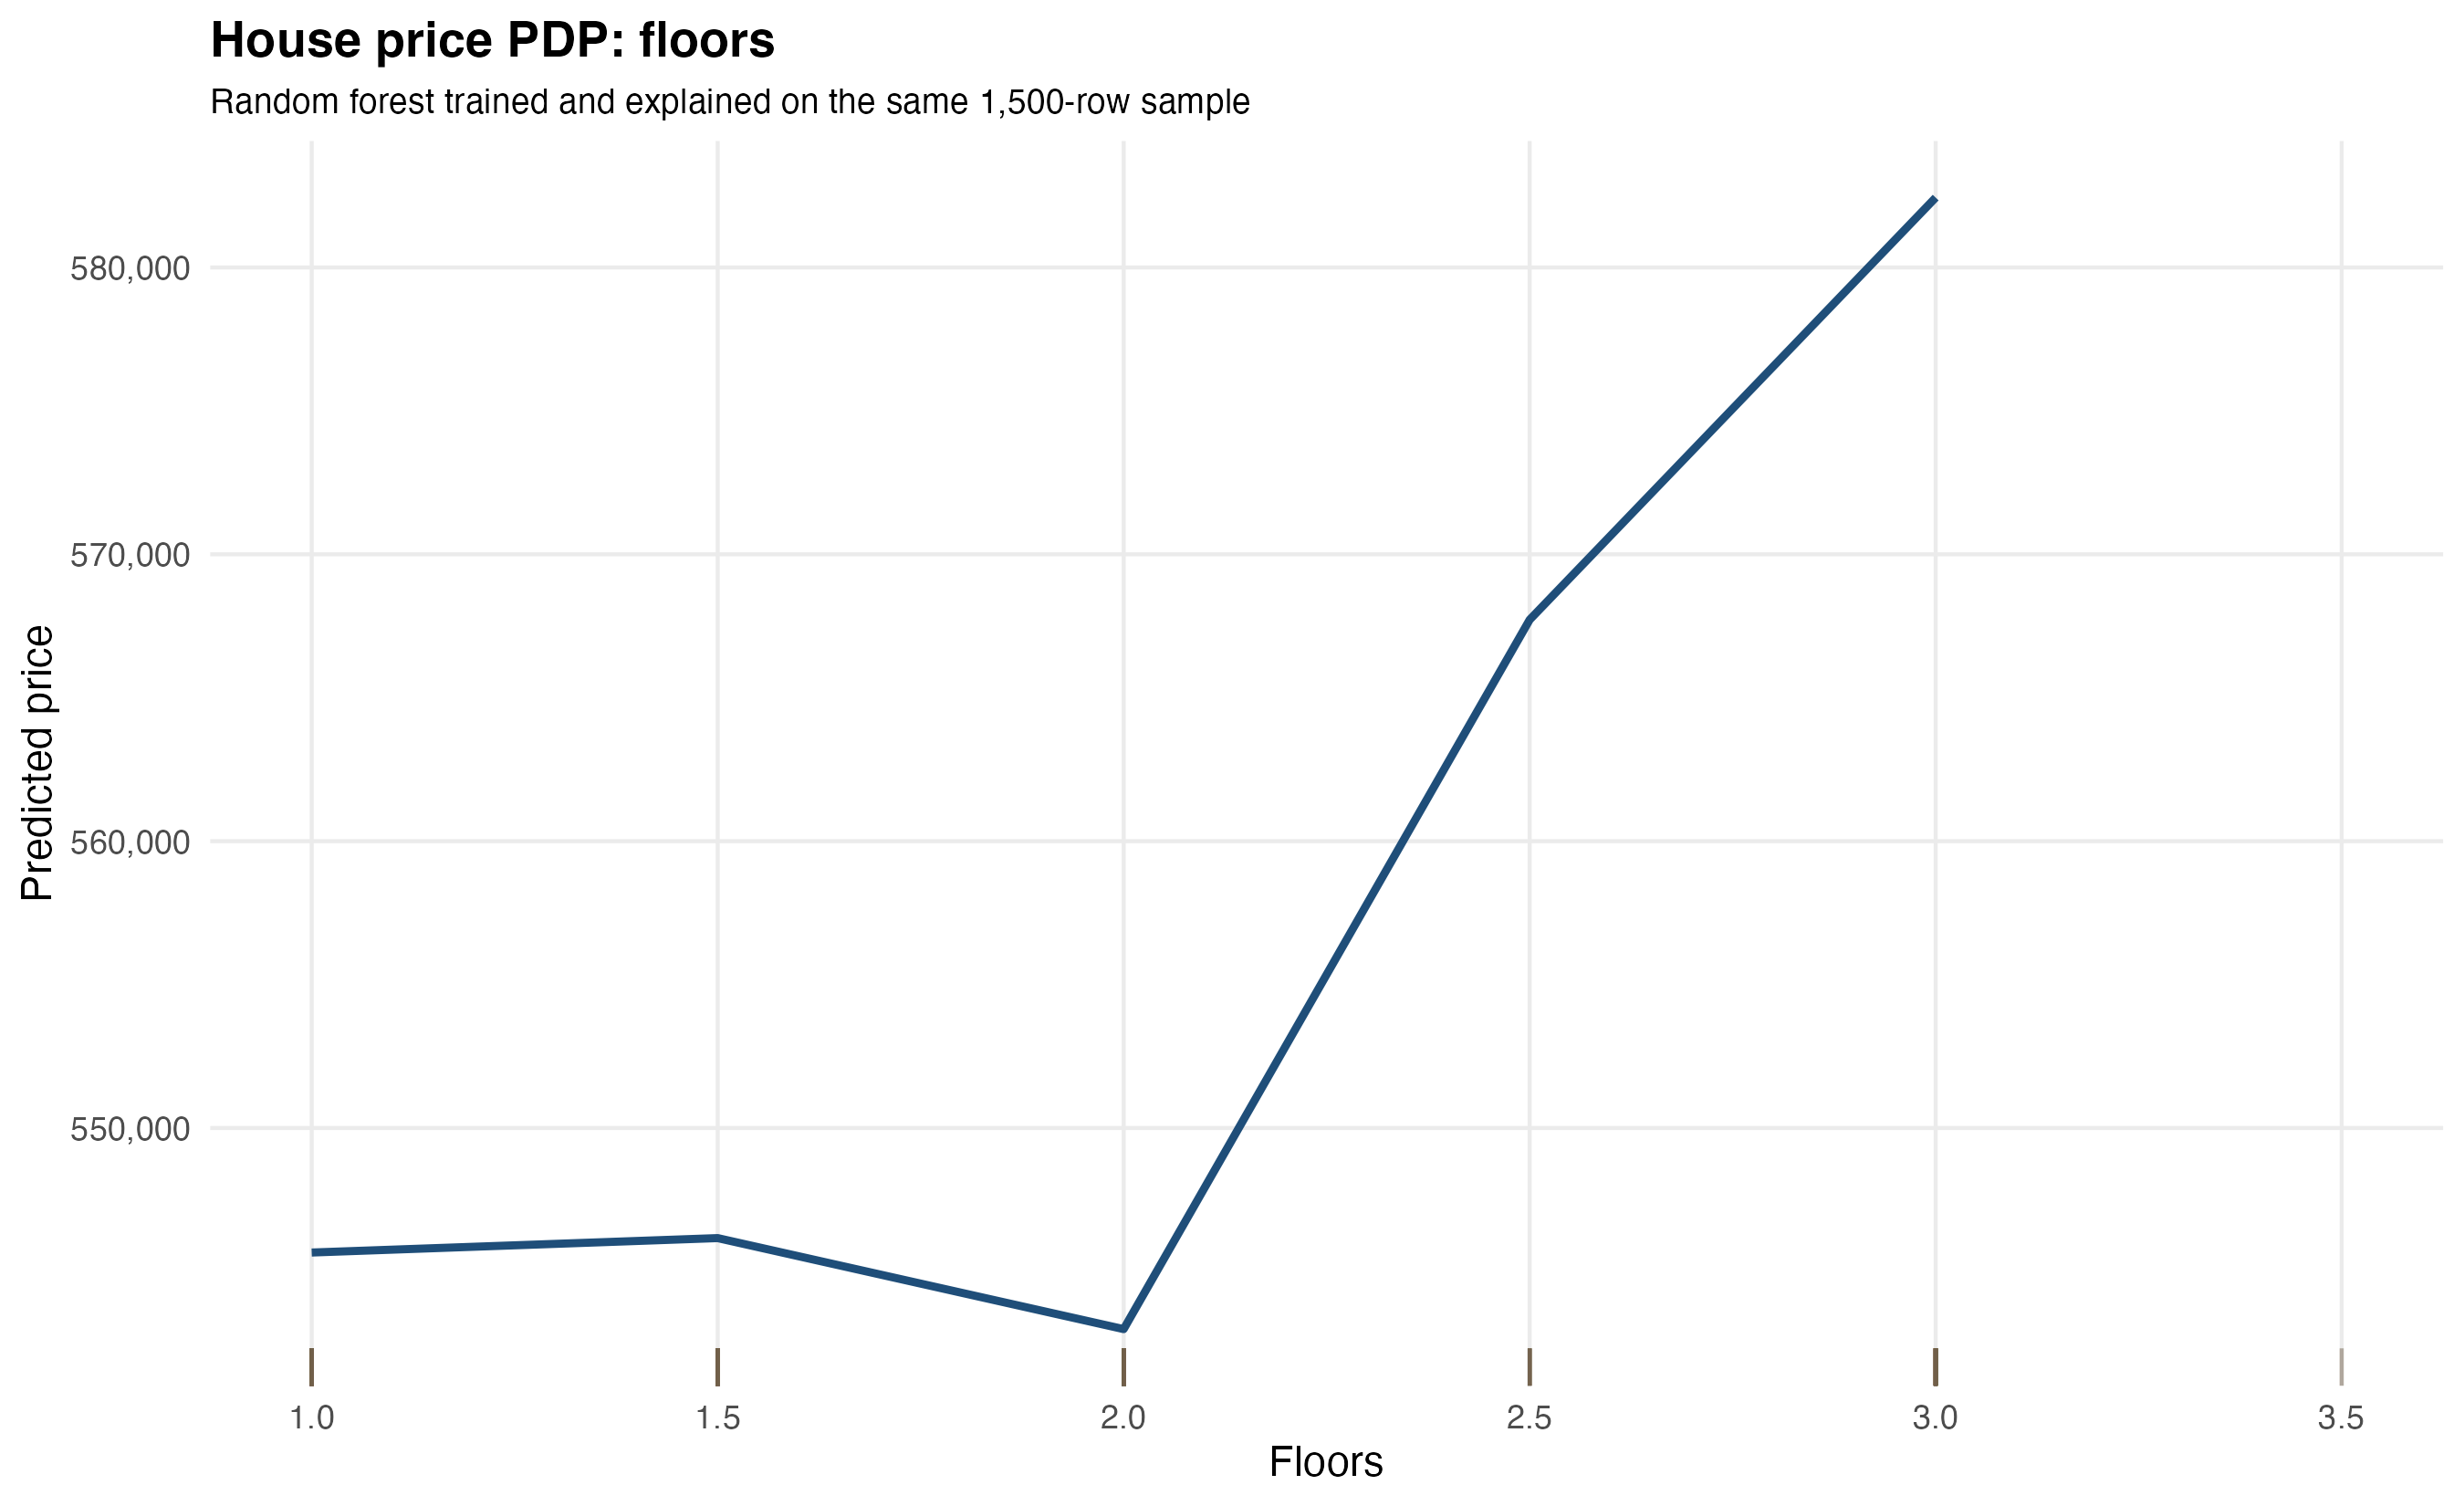
\includegraphics[width=\textwidth]{house_pdp_floors.png}
\end{minipage}
\caption{One-dimensional PDPs for house price prediction.}
\end{figure}

\textbf{Bedrooms.} Bedrooms do not show a simple positive relationship in this model. The PDP is highest for two bedrooms, about 555,413 dollars, and lower for larger bedroom counts, with about 528,635 dollars at six bedrooms. This does not mean bedrooms reduce market value causally. It means that, after living area and other structural variables are included, the number of bedrooms alone is not the main driver of the random forest prediction.

\textbf{Bathrooms.} Bathrooms have a positive model effect. Predicted price rises from about 486,756 dollars at one bathroom to about 712,858 dollars near 3.75 bathrooms. This is consistent with bathrooms acting as a quality and capacity signal.

\textbf{Living area.} Living area is the strongest house price driver. The PDP rises from about 340,102 dollars at 720 square feet to about 1,279,755 dollars near 3,975 square feet. For a real estate business, this is the clearest segmentation variable among the features used.

\textbf{Floors.} Floors have a moderate positive effect. The PDP rises from about 545,660 dollars at one floor to about 582,437 dollars at three floors. This effect is much smaller than living area, so it should be treated as a secondary driver.

\section{Recommendations}

\begin{itemize}
    \item Use normalized temperature, humidity, and wind speed as practical daily inputs for bike rental capacity planning.
    \item Treat medium-high normalized temperature and moderate normalized humidity as the strongest demand conditions for bikes.
    \item Lower bike staffing and fleet expectations on very humid or windy days, especially when temperature is low.
    \item For house pricing, prioritize living area in business explanations and customer-facing valuation discussions.
    \item Use bedrooms carefully. Bedroom count can be misleading when interpreted without living area and other structural features.
    \item Keep PDPs as model audit tools. They are valuable for explaining predictions, but they are not causal estimates.
\end{itemize}

\section{GitHub Repository Structure}

The repository is organized for reproducibility:
\begin{itemize}
    \item Code: \texttt{src/01\_pdp\_random\_forest.R}
    \item Figures: \texttt{outputs/figures/}
    \item Tables: \texttt{outputs/tables/}
    \item Report source and PDF: \texttt{report/main.tex} and \texttt{report/main.pdf}
    \item Assignment reference: \texttt{references/XAI3.pdf}
\end{itemize}

To reproduce the work, run:
\begin{verbatim}
Rscript src/01_pdp_random_forest.R
cd report
latexmk -pdf -interaction=nonstopmode -halt-on-error main.tex
\end{verbatim}

\section{Limitations}

PDPs average over the explanatory sample. When features are correlated, PDP grids can include combinations that are rare in the data. This matters for both datasets: weather variables can be seasonally correlated, and house variables such as bedrooms, bathrooms, floors, and living area are structurally correlated.

The house price model should not be used as a full valuation engine. It excludes important features such as neighborhood, condition, view, grade, renovation status, and sale timing. Its purpose here is to satisfy the assignment and provide a clear interpretability workflow.

\end{document}
